\documentclass[12pt]{ctexart}
\usepackage{amsmath} % 用于数学公式
\usepackage{graphicx} % 用于插入图片
\usepackage{listings} % 用于插入代码
\usepackage{float}    % 用于控制图表浮动位置

\usepackage{booktabs} % 用于创建更美观的三线表
\usepackage{siunitx}  % 用于标准地排版物理单位和数值
\usepackage{amsmath}  % 用于数学公式环境
\sisetup{per-mode=symbol} % 设置单位格式，例如 m/s

\usepackage{fancyhdr}   % 用于自定义页眉页脚
\usepackage{caption}   % 用于自定义图表标题
\usepackage{subcaption} % 用于子图环境
\usepackage[colorlinks, linkcolor=black]{hyperref}  % 用于创建超链接
\usepackage{makecell}
\usepackage{multirow}  

% \pdfcompresslevel=9

\graphicspath{{./figures/}}

\usepackage[left=2.5cm, right=2.5cm, top=2cm, bottom=2cm]{geometry}

\setlength{\jot}{6pt} % 增加多行公式之间的行距

\linespread{1.5}

\pagestyle{fancy}

\begin{document}

% \maketitle
\thispagestyle{empty}

\begin{figure}[t]
    \centering
    
\includegraphics[width=13cm]{./figures/logo1.png}
\end{figure}

\vspace*{\fill}
    \begin{center}
        \Huge\textbf{实验4：有源、无源滤波器}
    \end{center}
\vspace*{\fill}

\begin{table}[H]
    \centering
    \large
    \begin{tabular}{ll}
    \textbf{课程:} & 信号与系统实验 \\
    \textbf{姓名:} & 郭浩然 \\
    \textbf{学号:} & 2024303980 \\
    \textbf{桌号:} & 18 \\
    \textbf{班级:} & 10班 \\
    \textbf{学院:} & 民航学院 \\
    \textbf{专业:} & 飞行器控制与信息工程 \\
    \textbf{时间:} & \today \\
    \end{tabular}
\end{table}

\newpage

\tableofcontents
\newpage

% ==========================================
% 第一部分：实验目的、器材与原理
% ==========================================

\section{实验目的}

\begin{enumerate}
    \item 熟悉滤波器的构成及其特性（包括有源、无源；低通、高通、带通、带阻）。
    \item 学会测量滤波器幅频特性的方法（点频法与扫频法）。
\end{enumerate}

\section{实验器材}

\begin{enumerate}
    \item 双踪示波器 \quad 1台
    \item 信号源及频率计模块 (S2) \quad 1块
    \item 抽样定理及滤波器模块 (S3) \quad 1块
\end{enumerate}

\section{实验原理}

滤波器是一种能使有用频率信号通过而同时抑制（或大为衰减）无用频率信号的电子装置。工程上常用它作信号处理、数据传送和抑制干扰等。

本实验主要讨论模拟滤波器。
\begin{itemize}
    \item \textbf{无源滤波器}：主要采用无源元件 $R$、$L$ 和 $C$ 组成。
    \item \textbf{有源滤波器}：由集成运放和 $R$、$C$ 组成。具有不用电感、体积小、重量轻等优点，且具有一定的电压放大和缓冲作用，但带宽受运放限制。
\end{itemize}

\subsection{基本概念及初步定义}

滤波电路的一般结构如图 \ref{fig:filter_structure} 所示。设输入信号为 $V_{i}(t)$，输出信号为 $V_{o}(t)$。

\begin{figure}[htbp]
    \centering
    % 请确保图片路径正确，此处使用占位符，您可以使用您提供的原理图替换
    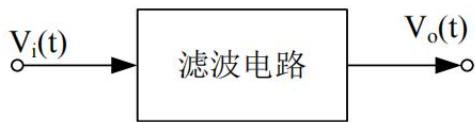
\includegraphics[width=0.6\textwidth]{figures/原理图1.png} 
    % \fbox{\parbox{0.6\textwidth}{\centering \vspace{2cm} 图 4-1 滤波器电路的一般结构 \vspace{2cm}}}
    \caption{滤波器电路的一般结构}
    \label{fig:filter_structure}
\end{figure}

假设滤波器是一个线性时不变网络，则在复频域内电压传递函数 $A(s)$ 定义为：
\begin{equation}
    A(s) = \frac{V_{o}(s)}{V_{i}(s)}
\end{equation}
对于实际频率（$s = j\omega$），则有：
\begin{equation}
    A(j\omega) = |A(j\omega)| e^{j\phi(\omega)}
\end{equation}
其中 $|A(j\omega)|$ 为幅频特性，$\phi(\omega)$ 为相频特性。

\subsection{各类滤波器的传输函数}

不同类型滤波器的理想传输函数及参数定义如表 \ref{tab:transfer_functions} 所示。

\begin{table}[htbp]
    \centering
    \caption{各类滤波器的传输函数及参数说明}
    \label{tab:transfer_functions}
    \renewcommand{\arraystretch}{2} % 增加行高，使公式更清晰
    \begin{tabular}{|c|c|l|}
        \hline
        \textbf{类型} & \textbf{传输函数} $A(s)$ & \multicolumn{1}{c|}{\textbf{备注}} \\
        \hline
        低通 & $\displaystyle \frac{A_V \omega_c^2}{s^2 + \frac{\omega_c}{Q}s + \omega_c^2}$ & \multirow{4}{*}{\makecell[l]{$A_V$ —— 电压增益 \\ $\omega_c$ —— 低、高通滤波器的截止角频率 \\ $\omega_o$ —— 带通、带阻滤波器的中心角频率 \\ $Q$ —— 品质因数 \\ $BW$ —— 带宽 \\ $Q \approx \frac{\omega_o}{BW}$ (当 $BW \ll \omega_o$ 时)}} \\
        \cline{1-2}
        高通 & $\displaystyle \frac{A_V s^2}{s^2 + \frac{\omega_c}{Q}s + \omega_c^2}$ & \\
        \cline{1-2}
        带通 & $\displaystyle \frac{A_V \frac{\omega_o}{Q}s}{s^2 + \frac{\omega_o}{Q}s + \omega_o^2}$ & \\
        \cline{1-2}
        带阻 & $\displaystyle \frac{A_V (s^2 + \omega_o^2)}{s^2 + \frac{\omega_o}{Q}s + \omega_o^2}$ & \\
        \hline
    \end{tabular}
\end{table}

\subsection{滤波电路的分类与幅频响应}

根据幅频响应，滤波电路通常分为以下四类（如图 \ref{fig:freq_response} 所示）：

\begin{enumerate}
    \item \textbf{低通 (LPF)}：通带 $0 \sim \omega_H$，截止频率 $BW = \omega_H$。
    \item \textbf{高通 (HPF)}：通带 $\omega > \omega_L$。
    \item \textbf{带通 (BPF)}：通带 $\omega_L \sim \omega_H$，带宽 $BW = \omega_H - \omega_L$。
    \item \textbf{带阻 (BEF)}：阻带 $\omega_H \sim \omega_L$，中心频率 $\omega_o$。
\end{enumerate}

\begin{figure}[htbp]
    \centering
    \begin{subfigure}{0.35\textwidth}
        \centering
        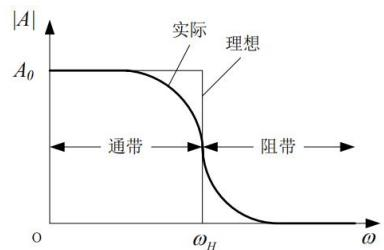
\includegraphics[width=\textwidth]{figures/lpf.png}
        \caption{低通滤波器 LPF}
    \end{subfigure}
    % \hfill
    \begin{subfigure}{0.35\textwidth}
        \centering
        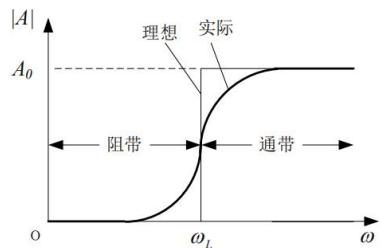
\includegraphics[width=\textwidth]{figures/hpf.png}
        \caption{高通滤波器 HPF}
    \end{subfigure}

    \vspace{0.5cm}

    \begin{subfigure}{0.35\textwidth}
        \centering
        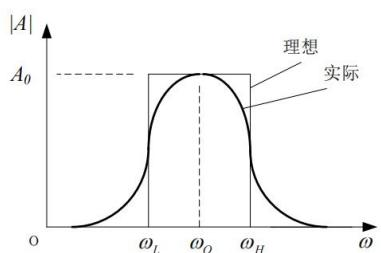
\includegraphics[width=\textwidth]{figures/bpf.png}
        \caption{带通滤波器 BPF}
    \end{subfigure}
    % \hfill
    \begin{subfigure}{0.35\textwidth}
        \centering
        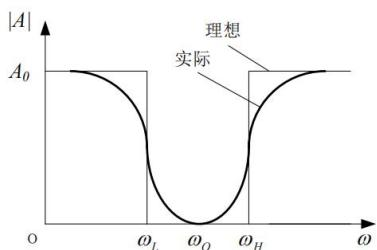
\includegraphics[width=\textwidth]{figures/bef.png}
        \caption{带阻滤波器 BEF}
    \end{subfigure}

    \caption{各种滤波电路的幅频响应}
    \label{fig:freq_response}
\end{figure}

\section{实验步骤}

实验中信号源的输入信号均为 $4\,\mathrm{V}$ 左右的正弦波。

\textbf{设置模块}：按下波形切换 S4，使“SIN”指示灯亮，调节“模拟输出幅度调节”旋钮，使信号幅度为 $4\,\mathrm{V}$。

% ---------------------------------------------------------
% 任务一
% ---------------------------------------------------------
\subsection{任务一：测量低通滤波器的频响特性}

\subsubsection{逐点测量法（点频法）}

\begin{enumerate}
    \item 模块关电，连接模块 S2 中模拟信号输出端 P2 与模块 S3 中 P1（低通无源），保持输入信号幅度为 $4\,\mathrm{V}$ 不变。
    
    \begin{figure}[htbp]
        \centering
        % 如果您有接线图，请取消注释并修改文件名；如果没有，请删除此figure块
        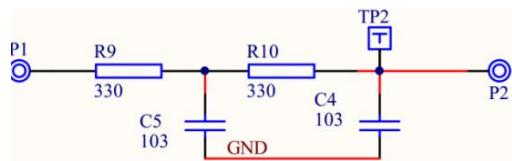
\includegraphics[width=0.6\textwidth]{figures/原理图_无源低通.png} 
        % \fbox{\parbox{0.6\textwidth}{\centering \vspace{1.5cm} 此处插入：图 4-3 (a) 无源低通滤波器接线图 \vspace{1.5cm}}}
        \caption{无源低通滤波器接线示意}
    \end{figure}

    \item 模块开电，逐渐改变输入信号频率，并用示波器观测 TP2 处信号波形的峰峰值。
    \item 将数据记录（后续填入数据分析章节的表中）。
    \item 连接模块 S2 中模拟信号输出端 P2 与模块 S3 中 P5（低通有源）。
    \item 逐渐改变输入信号频率，并用示波器观测 TP6 处信号波形的峰峰值。
    \item 将数据记录。
    
    \begin{figure}[htbp]
        \centering
        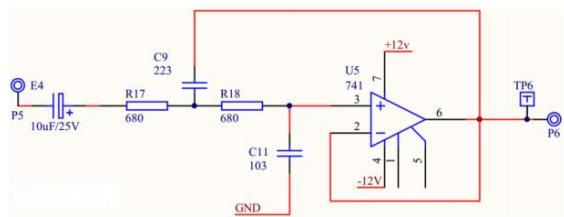
\includegraphics[width=0.6\textwidth]{figures/原理图_有源低通.png}
        % \fbox{\parbox{0.6\textwidth}{\centering \vspace{1.5cm} 此处插入：图 4-3 (b) 有源低通滤波器接线图 \vspace{1.5cm}}}
        \caption{有源低通滤波器接线示意}
    \end{figure}
\end{enumerate}

\subsubsection{扫频法测量}

\textbf{原理}：S2 模块产生扫频信号，当它经过滤波器后，对比分析输入和输出的信号频率，就可以知道滤波器的特性。

\textbf{步骤}：
\begin{enumerate}
    \item 将扫频范围设置为 $100\,\mathrm{Hz} \sim 35\,\mathrm{kHz}$。
    \item 把示波器连接到信号源上输出 P2 处（示波器调为直流测试档），此时点 P2 输出扫频信号。
    \item 模块关电，分别把 S2 中 P2 输出的扫频信号输入到模块 S3 低通滤波器的输入端 P1（无源）或 P5（有源）。
    \item 模块开电，示波器另一通道接输出，拍照记录此时示波器上的输入输出信号。
\end{enumerate}

% ---------------------------------------------------------
% 任务二
% ---------------------------------------------------------
\subsection{任务二：测量高通滤波器的频响特性}

\subsubsection{逐点测量法（点频法）}

\begin{enumerate}
    \item 模块关电，保持信号源输出的正弦信号幅度不变，连接模块 S2 中模拟信号源部分 P2 与模块 S3 中模拟滤波器中的 P3（高通无源）端口。
    
    \begin{figure}[htbp]
        \centering
        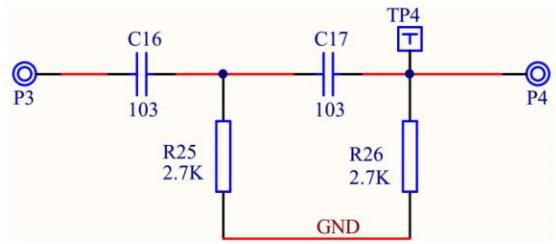
\includegraphics[width=0.6\textwidth]{figures/原理图_无源高通.png}
        % \fbox{\parbox{0.6\textwidth}{\centering \vspace{1.5cm} 此处插入：图 5-4 (a) 高通无源滤波器接线图 \vspace{1.5cm}}}
        \caption{高通无源滤波器接线示意}
    \end{figure}

    \item 模块开电，逐渐改变输入信号频率，并用示波器观测 TP4 处信号波形的峰峰值。
    \item 将数据记录。
    \item 模块关电，连接模块 S3 中模拟信号输出端 P2 与模块 S3 中模拟滤波器中的 P7（高通有源）。
    
    \begin{figure}[htbp]
        \centering
        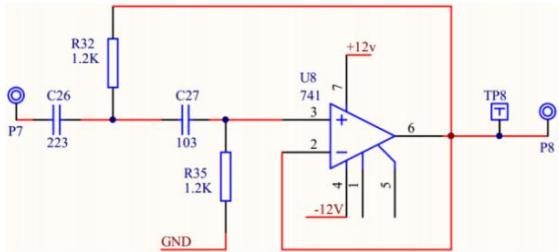
\includegraphics[width=0.6\textwidth]{figures/原理图_有源高通.png}
        % \fbox{\parbox{0.6\textwidth}{\centering \vspace{1.5cm} 此处插入：图 5-4 (b) 高通有源滤波器接线图 \vspace{1.5cm}}}
        \caption{高通有源滤波器接线示意}
    \end{figure}

    \item 模块开电，逐渐改变输入信号频率，并用示波器观测 TP8 处信号波形的峰峰值。
    \item 将数据记录。
\end{enumerate}

\subsubsection{扫频法测量}

将扫频范围设置为 $100\,\mathrm{Hz} \sim 35\,\mathrm{kHz}$，把示波器连接到信号源上输出 P2 处（示波器调为直流测试档），此时点 P2 输出扫频信号。模块关电，把扫频信号输入到高通滤波器的输入端，模块开电，拍照记录此时的输入输出信号。

% ---------------------------------------------------------
% 任务三
% ---------------------------------------------------------
\subsection{任务三：测量带通滤波器的频响特性}

\subsubsection{逐点测量法}

\begin{enumerate}
    \item 模块关电，保持信号源输出的正弦信号幅度不变，连接模块 S2 中 P2 与模块 S3 中模拟滤波器中的 P9 相连（带通无源）。
    
    \begin{figure}[htbp]
        \centering
        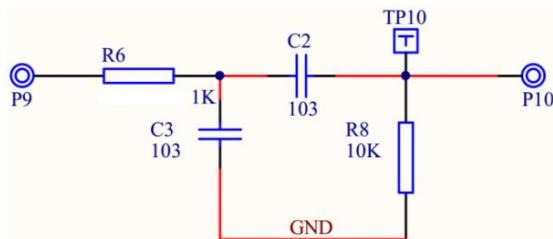
\includegraphics[width=0.6\textwidth]{figures/原理图_无源带通.png}
        % \fbox{\parbox{0.6\textwidth}{\centering \vspace{1.5cm} 此处插入：图 4-5 (a) 带通无源滤波器接线图 \vspace{1.5cm}}}
        \caption{带通无源滤波器接线示意}
    \end{figure}

    \item 模块开电，逐渐改变输入信号频率，并用示波器观测 TP10 处信号波形的峰峰值。
    \item 将数据记录。
    \item 模块关电，保持信号源输出的正弦波幅度为 $4\,\mathrm{V}$ 不变，连接模块 S2 中 P2 与模块 S3 中模拟滤波器中的 P13（带通有源）。
    \item 模块开电，逐渐改变输入信号频率，并用示波器观测 TP14 处信号波形的峰峰值。
    \item 将数据记录。
\end{enumerate}

\subsubsection{扫频法测量}

将扫频范围设置为 $100\,\mathrm{Hz} \sim 35\,\mathrm{kHz}$，把示波器连接到信号源上输出 P2 处（示波器调为直流测试档），此时点 P2 输出扫频信号。把扫频信号输入到带通滤波器的输入端，拍照记录此时的输入输出信号。

% ---------------------------------------------------------
% 任务四
% ---------------------------------------------------------
\subsection{任务四：测量带阻滤波器的频响特性}

\subsubsection{逐点测量法}

\begin{enumerate}
    \item 模块关电，保持信号源输出的正弦信号幅度不变，连接模块 S2 中 P2 与模块 S3 中模拟滤波器中的 P11（带阻无源）。
    \item 模块开电，逐渐改变输入信号频率，并用示波器观测 TP12 处信号波形的峰峰值。
    \item 将数据记录。
    
    \begin{figure}[htbp]
        \centering
        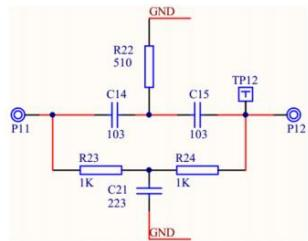
\includegraphics[width=0.6\textwidth]{figures/原理图_无源带阻.png}
        % \fbox{\parbox{0.6\textwidth}{\centering \vspace{1.5cm} 此处插入：图 4-6 (a) 带阻无源滤波器接线图 \vspace{1.5cm}}}
        \caption{带阻无源滤波器接线示意}
    \end{figure}

    \item 模块关电，保持信号源输出的正弦信号幅度 $4\,\mathrm{V}$ 不变，连接模块 S2 中 P2 与模块 S3 中模拟滤波器中的 P15（带阻有源）。
    
    \begin{figure}[htbp]
        \centering
        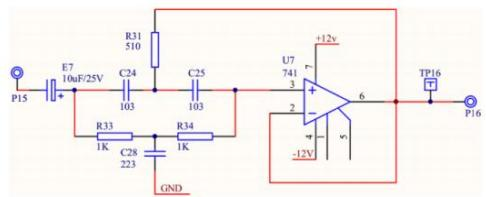
\includegraphics[width=0.6\textwidth]{figures/原理图_有源带阻.png}
        % \fbox{\parbox{0.6\textwidth}{\centering \vspace{1.5cm} 此处插入：图 4-6 (b) 带阻有源滤波器接线图 \vspace{1.5cm}}}
        \caption{带阻有源滤波器接线示意}
    \end{figure}

    \item 模块开电，逐渐改变输入信号频率，并用示波器观测 TP16 处信号波形的峰峰值。
    \item 将数据记录。
\end{enumerate}

\subsubsection{扫频法测量}

将扫频范围设置为 $100\,\mathrm{Hz} \sim 80\,\mathrm{kHz}$，把示波器连接到信号源上输出 P2 处（示波器调为直流测试档），此时点 P2 输出扫频信号。模块关电，把扫频信号输入到带阻滤波器的输入端，模块开电，对比观察输入输出信号。



\section{实验记录与数据分析}

% 定义通用表格命令，包含 resizebox 以防止表格超宽
\newcommand{\mygridtable}[2]{
    \begin{table}[H]
        \centering
        \renewcommand{\arraystretch}{1.4} % 增加行高
        \setlength{\tabcolsep}{3pt}       % 减小列间距
        % 使用 resizebox 强制表格适应文本宽度，避免拆分
        \resizebox{\textwidth}{!}{
            #1
        }
        \caption{#2}
    \end{table}
}

% ---------------------------------------------------------
% 任务一：低通滤波器
% ---------------------------------------------------------
\subsection{任务一：测量低通滤波器的频响特性}

\subsubsection{逐点测量法数据}

\textbf{1. 无源低通滤波器}

\mygridtable{
    \begin{tabular}{|c|c|c|c|c|c|c|c|c|c|c|c|}
        \hline
        $V_i$ (V) & 4 & 4 & 4 & 4 & 4 & 4 & 4 & 4 & 4 & 4 & 4 \\
        \hline
        $f$ (Hz) & 100 & 1k & 5k & 10k & 15k & \textbf{18.5k} & 20k & 25k & 30k & 50k & 100k \\
        \hline
        $V_o$ (V) & 3.84 & 3.84 & 3.84 & 3.44 & 3.04 & \textbf{2.80} & 2.72 & 2.40 & 2.08 & 1.36 & 0.72 \\
        \hline
        \multicolumn{12}{|l|}{\textbf{测量结论：} 当 $V_o \approx 0.707 V_i \approx 2.828\,\mathrm{V}$ 时，测得截止频率 $f_H = 18.5\,\mathrm{kHz}$} \\
        \hline
    \end{tabular}
}{低通无源滤波器逐点测量数据}

\textbf{2. 有源低通滤波器}

\mygridtable{
    \begin{tabular}{|c|c|c|c|c|c|c|c|c|c|c|c|}
        \hline
        $V_i$ (V) & 4 & 4 & 4 & 4 & 4 & 4 & 4 & 4 & 4 & 4 & 4 \\
        \hline
        $f$ (Hz) & 100 & 1k & 5k & 10k & \textbf{16.7k} & 17k & 20k & 25k & 30k & 50k & 100k \\
        \hline
        $V_o$ (V) & 3.84 & 3.84 & 3.84 & 3.68 & \textbf{2.80} & 2.72 & 2.24 & 1.60 & 1.28 & 0.56 & 0.24 \\
        \hline
        \multicolumn{12}{|l|}{\textbf{测量结论：} 当 $V_o \approx 0.707 V_i \approx 2.828\,\mathrm{V}$ 时，测得截止频率 $f_H = 16.7\,\mathrm{kHz}$} \\
        \hline
    \end{tabular}
}{低通有源滤波器逐点测量数据}

\subsubsection{幅频特性曲线与扫频测试}

\begin{figure}[H]
    \centering
    \begin{subfigure}[b]{0.8\textwidth}
        \centering
        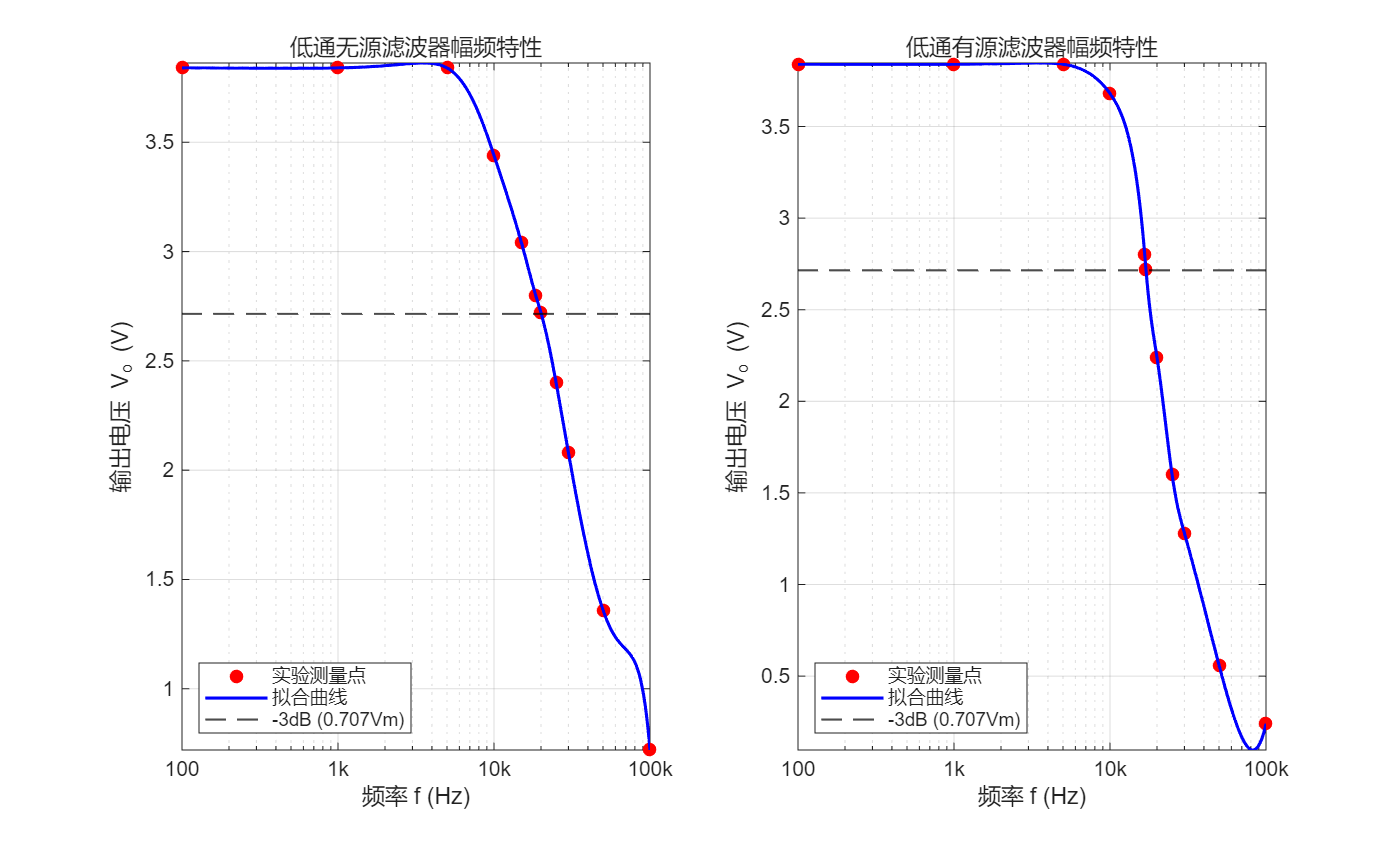
\includegraphics[width=\textwidth]{figures/低通.png}
        \caption{低通滤波器幅频特性曲线 (MATLAB)}
    \end{subfigure}
    
    \vspace{1em}
    
    \begin{subfigure}[b]{0.45\textwidth}
        \centering
        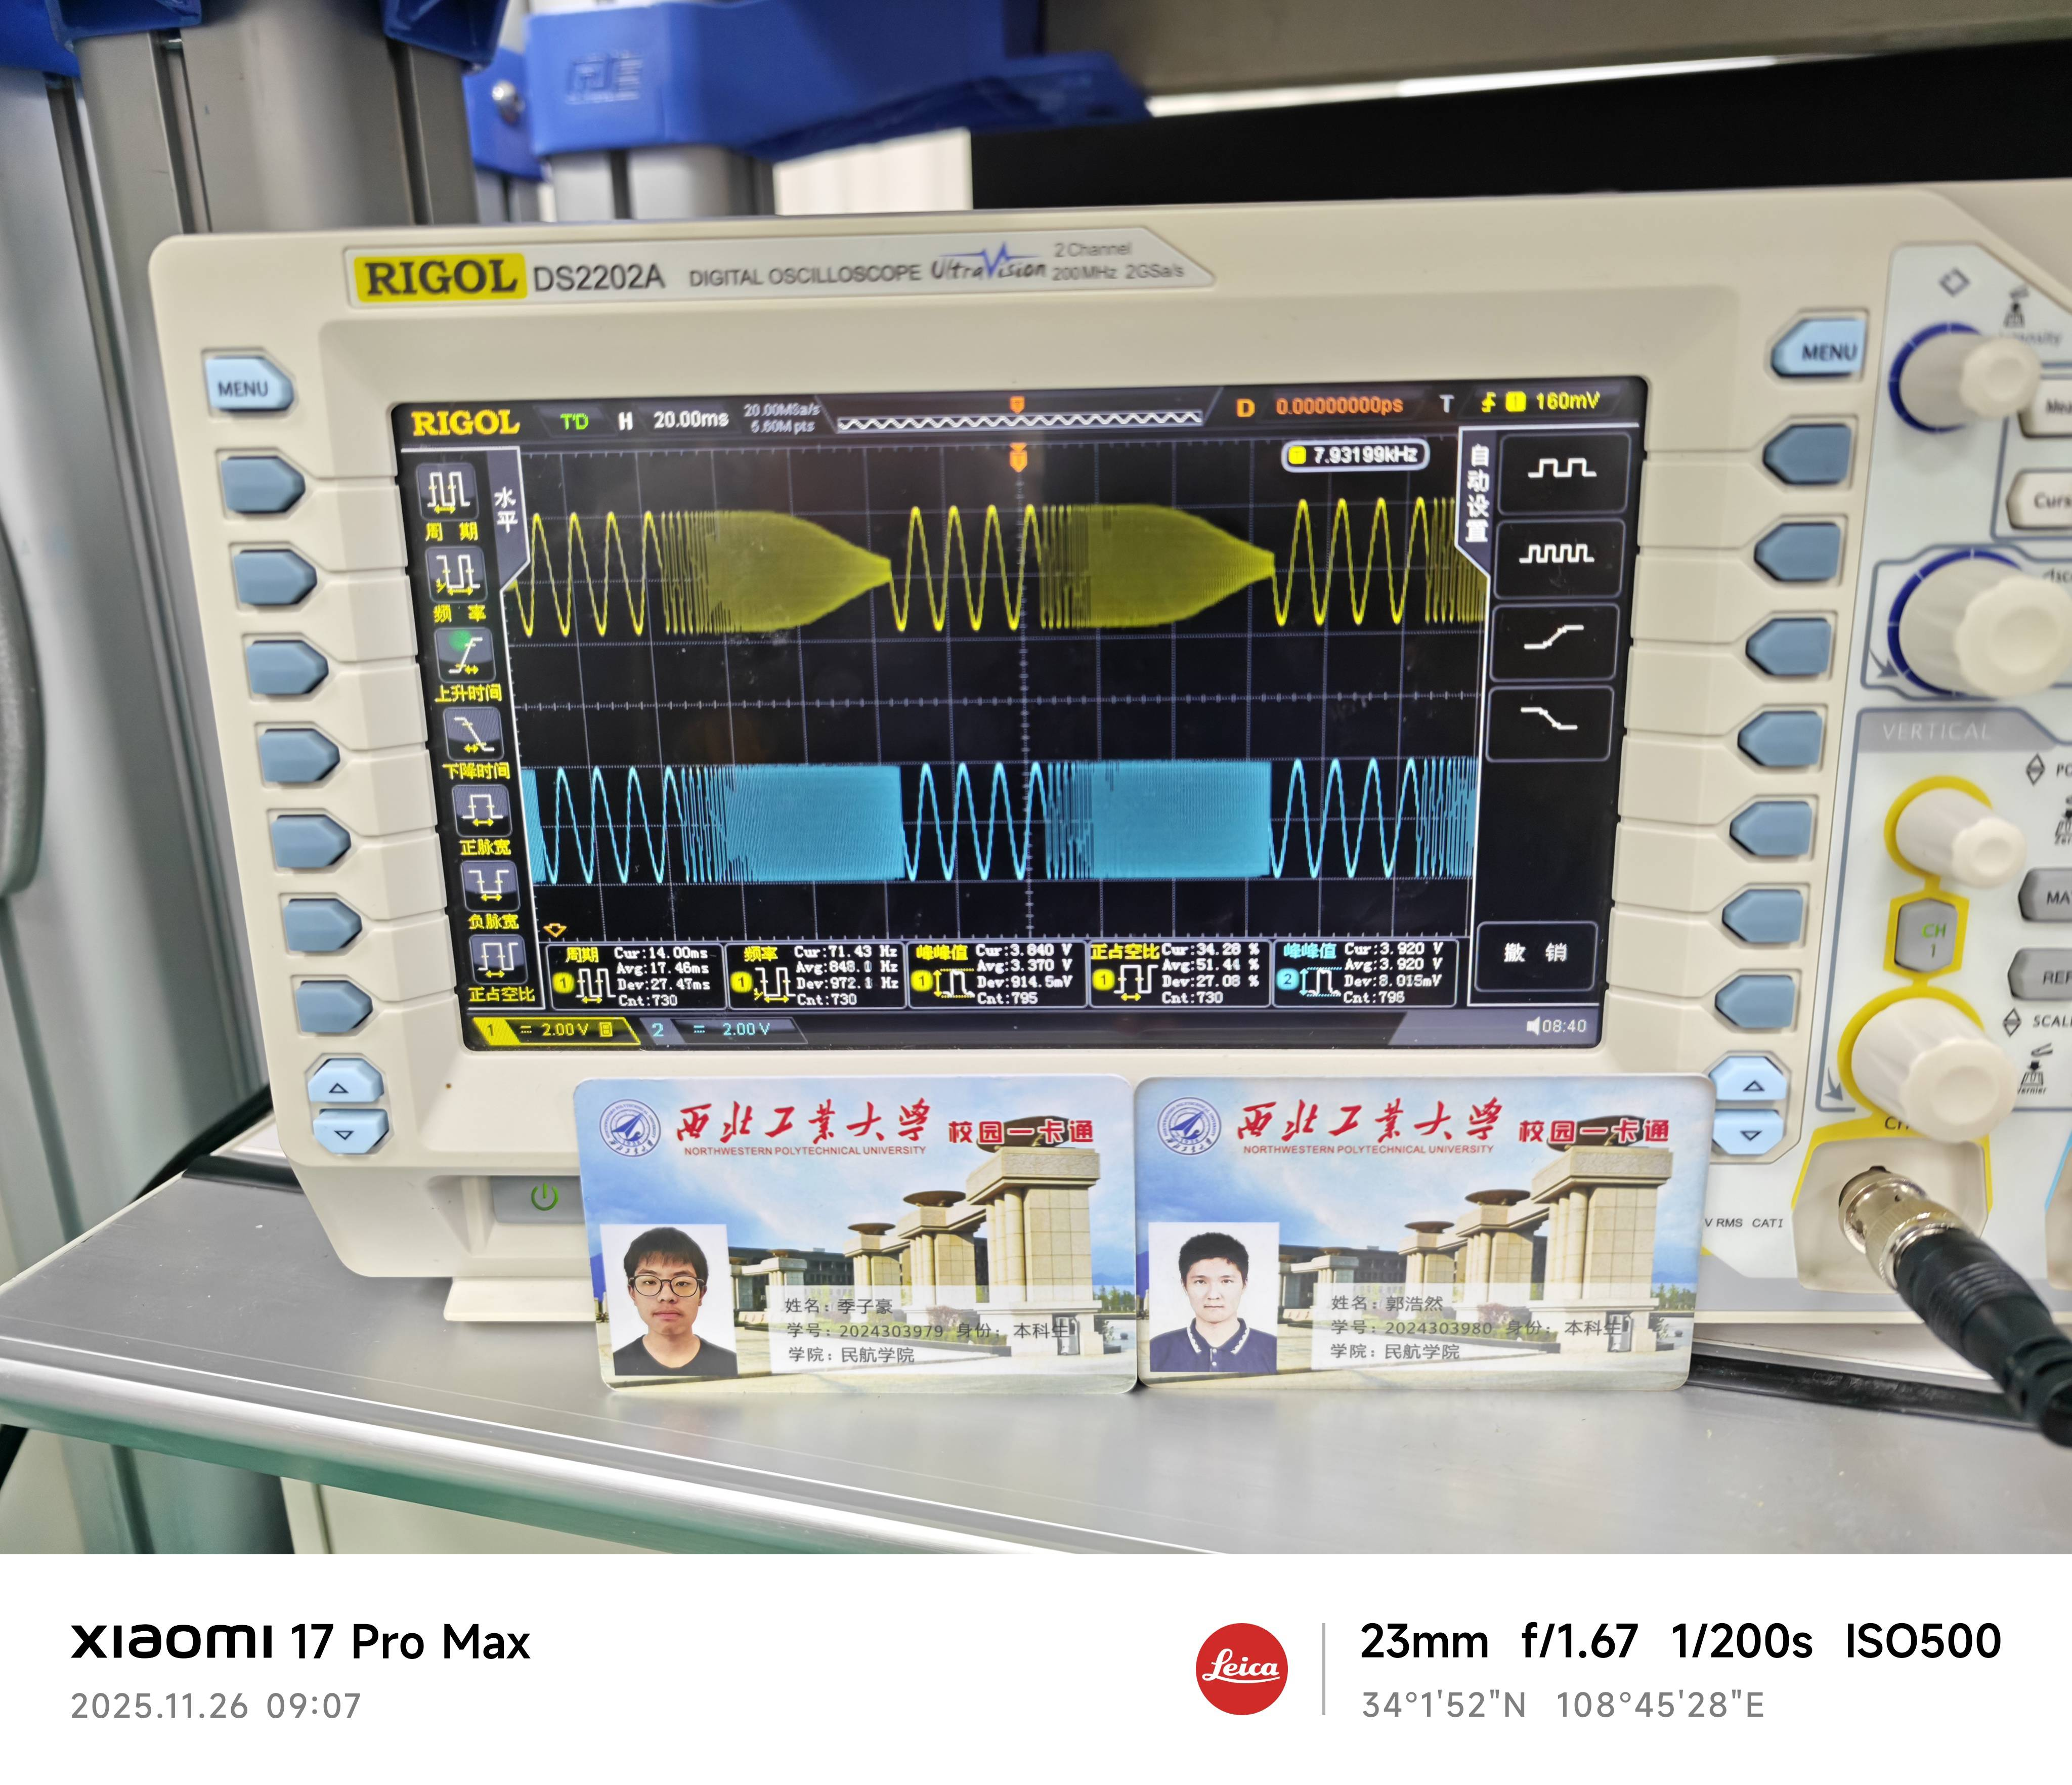
\includegraphics[width=\textwidth]{figures/无源低通.jpg}
        \caption{无源低通扫频波形}
    \end{subfigure}
    \hfill
    \begin{subfigure}[b]{0.45\textwidth}
        \centering
        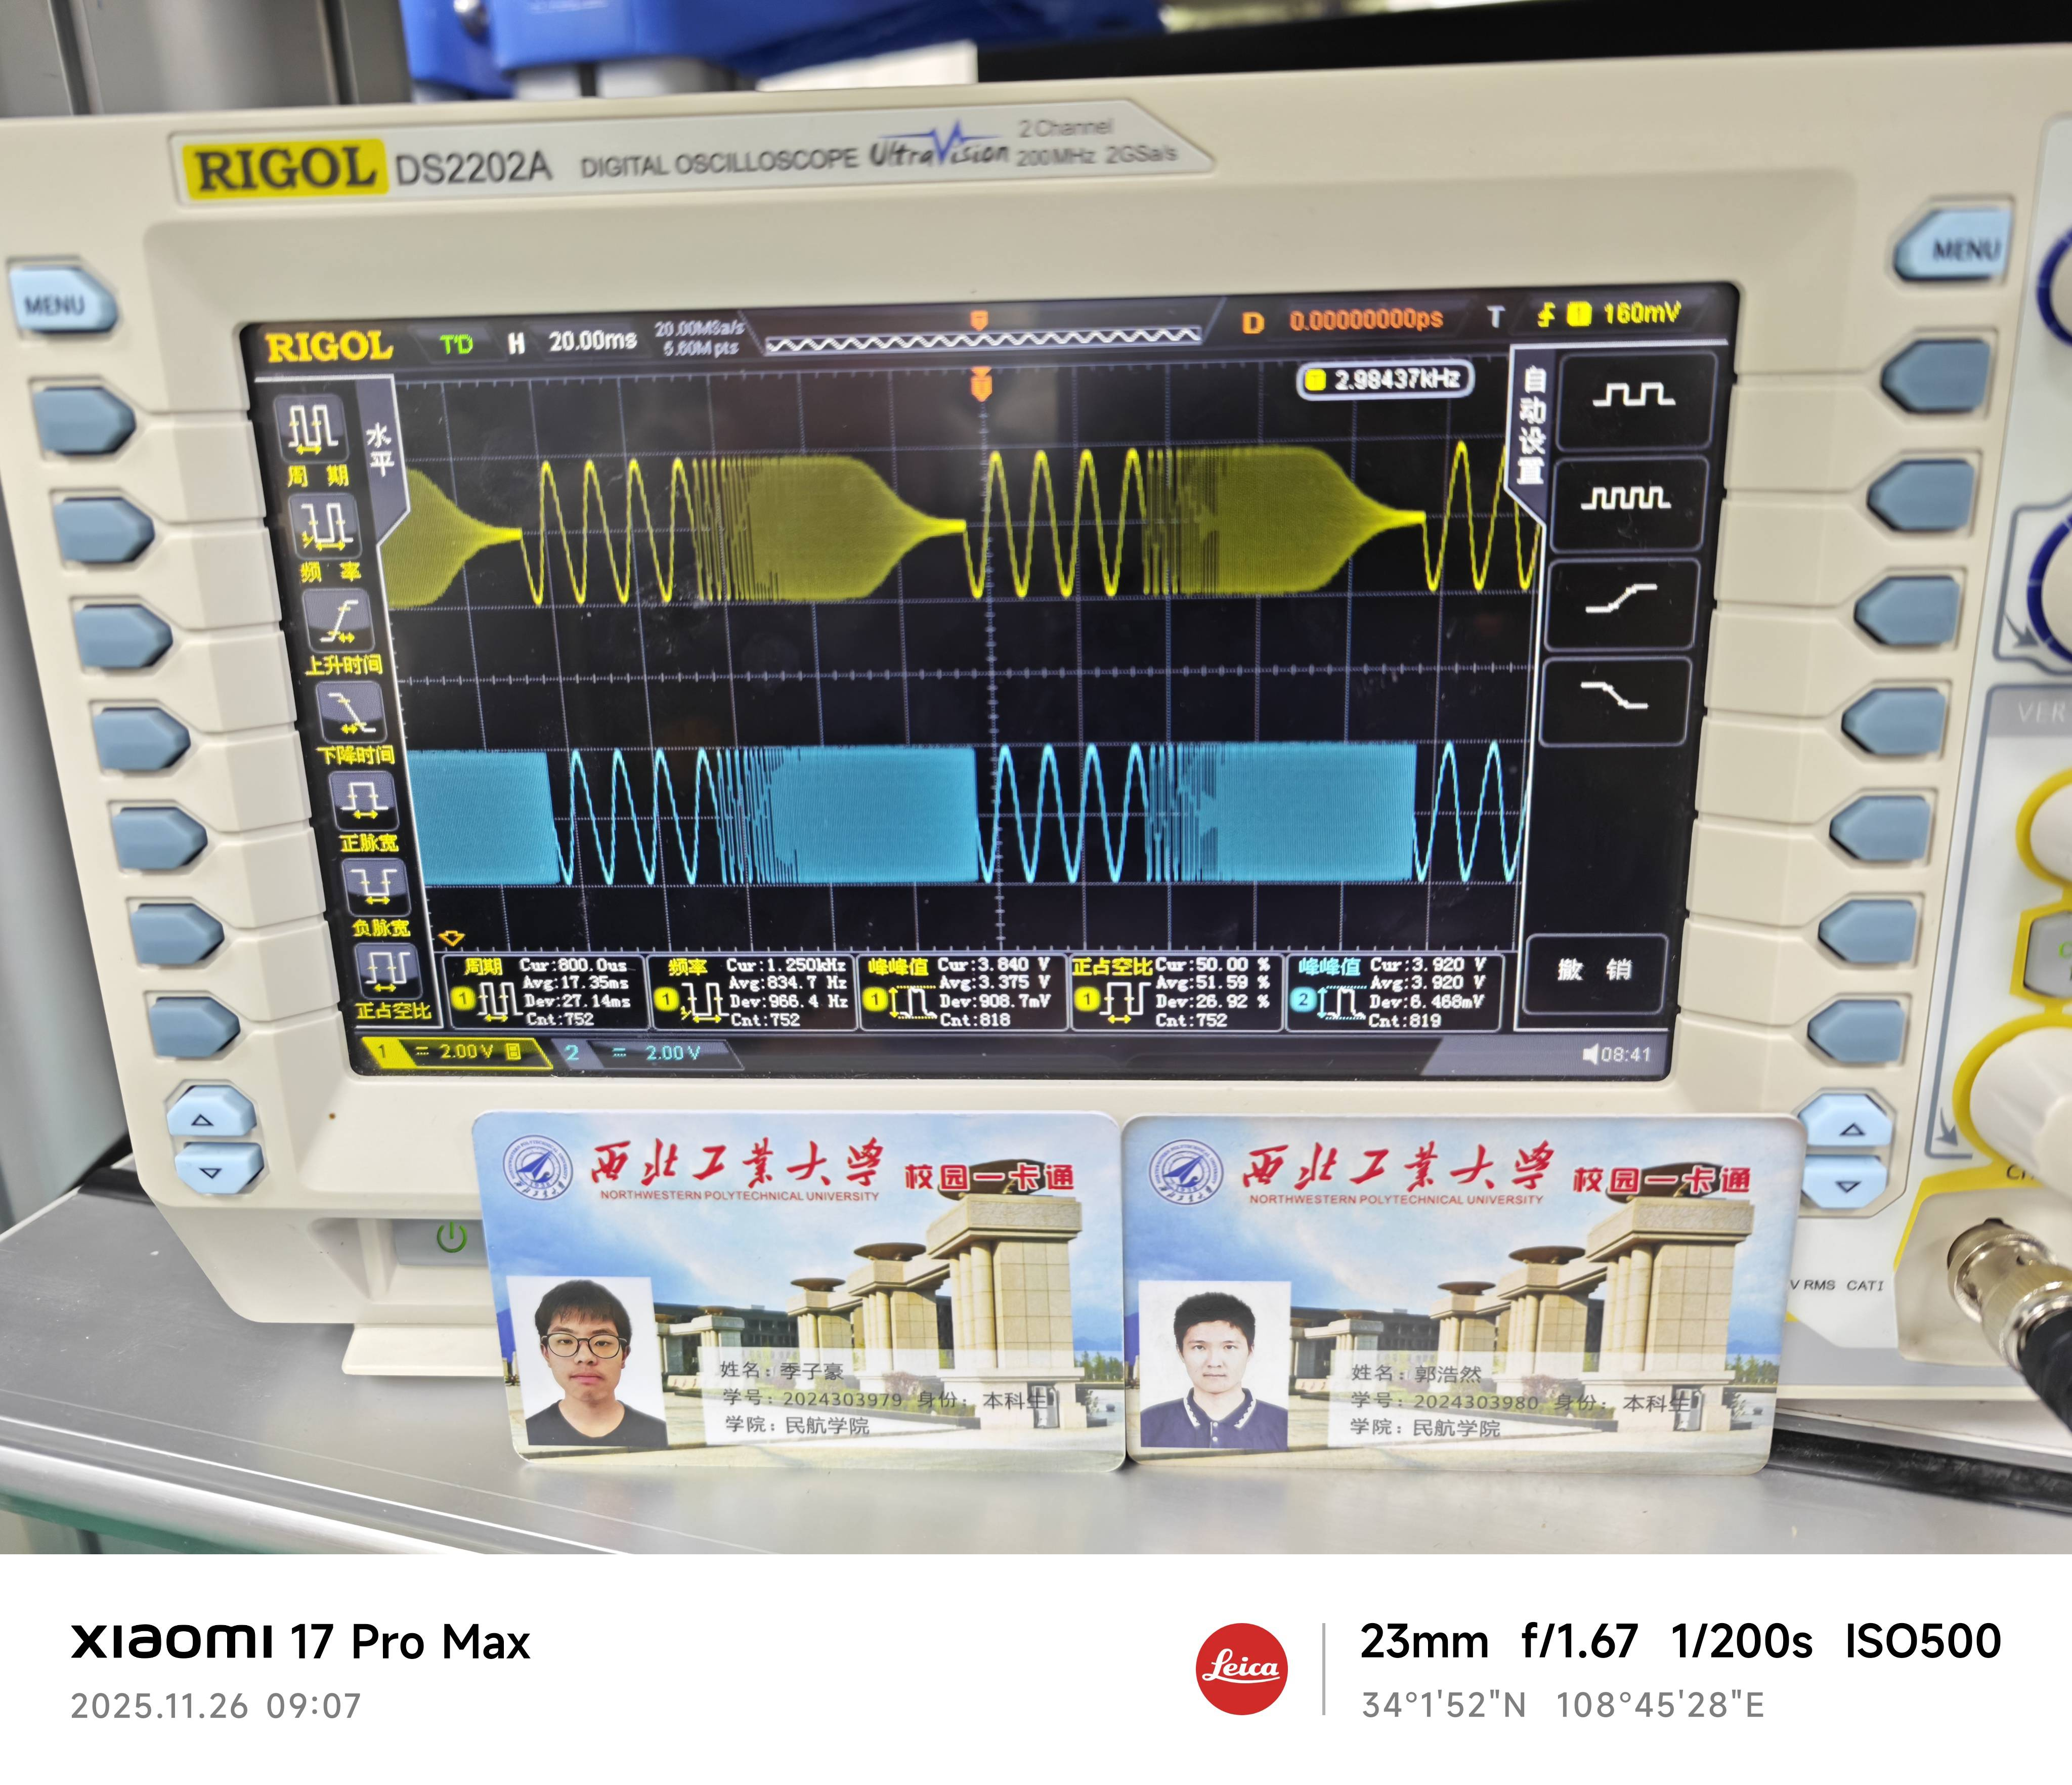
\includegraphics[width=\textwidth]{figures/有源低通.jpg}
        \caption{有源低通扫频波形}
    \end{subfigure}
    \caption{低通滤波器实验结果综合展示}
\end{figure}

\newpage

% ---------------------------------------------------------
% 任务二：高通滤波器
% ---------------------------------------------------------
\subsection{任务二：测量高通滤波器的频响特性}

\subsubsection{逐点测量法数据}

\textbf{1. 无源高通滤波器}

\mygridtable{
    \begin{tabular}{|c|c|c|c|c|c|c|c|c|c|c|c|}
        \hline
        $V_i$ (V) & 4 & 4 & 4 & 4 & 4 & 4 & 4 & 4 & 4 & 4 & 4 \\
        \hline
        $f$ (Hz) & 100 & 1k & 5k & 10k & 15k & \textbf{17.2k} & 20k & 25k & 30k & 50k & 100k \\
        \hline
        $V_o$ (V) & 0.24 & 0.24 & 1.20 & 2.00 & 2.64 & \textbf{2.80} & 2.96 & 3.12 & 3.28 & 3.52 & 3.60 \\
        \hline
        \multicolumn{12}{|l|}{\textbf{测量结论：} 当 $V_o \approx 2.828\,\mathrm{V}$ 时，测得截止频率 $f_L = 17.2\,\mathrm{kHz}$} \\
        \hline
    \end{tabular}
}{高通无源滤波器逐点测量数据}

\textbf{2. 有源高通滤波器}

\mygridtable{
    \begin{tabular}{|c|c|c|c|c|c|c|c|c|c|c|c|}
        \hline
        $V_i$ (V) & 4 & 4 & 4 & 4 & 4 & 4 & 4 & 4 & 4 & 4 & 4 \\
        \hline
        $f$ (Hz) & 100 & 1k & 5k & 10k & 15k & \textbf{17.0k} & 20k & 25k & 30k & 50k & 100k \\
        \hline
        $V_o$ (V) & 0.24 & 0.24 & 0.88 & 2.00 & 2.64 & \textbf{2.80} & 2.96 & 3.20 & 3.28 & 3.52 & 3.60 \\
        \hline
        \multicolumn{12}{|l|}{\textbf{测量结论：} 当 $V_o \approx 2.828\,\mathrm{V}$ 时，测得截止频率 $f_L = 17.0\,\mathrm{kHz}$} \\
        \hline
    \end{tabular}
}{高通有源滤波器逐点测量数据}

\subsubsection{幅频特性曲线与扫频测试}

\begin{figure}[H]
    \centering
    \begin{subfigure}[b]{0.8\textwidth}
        \centering
        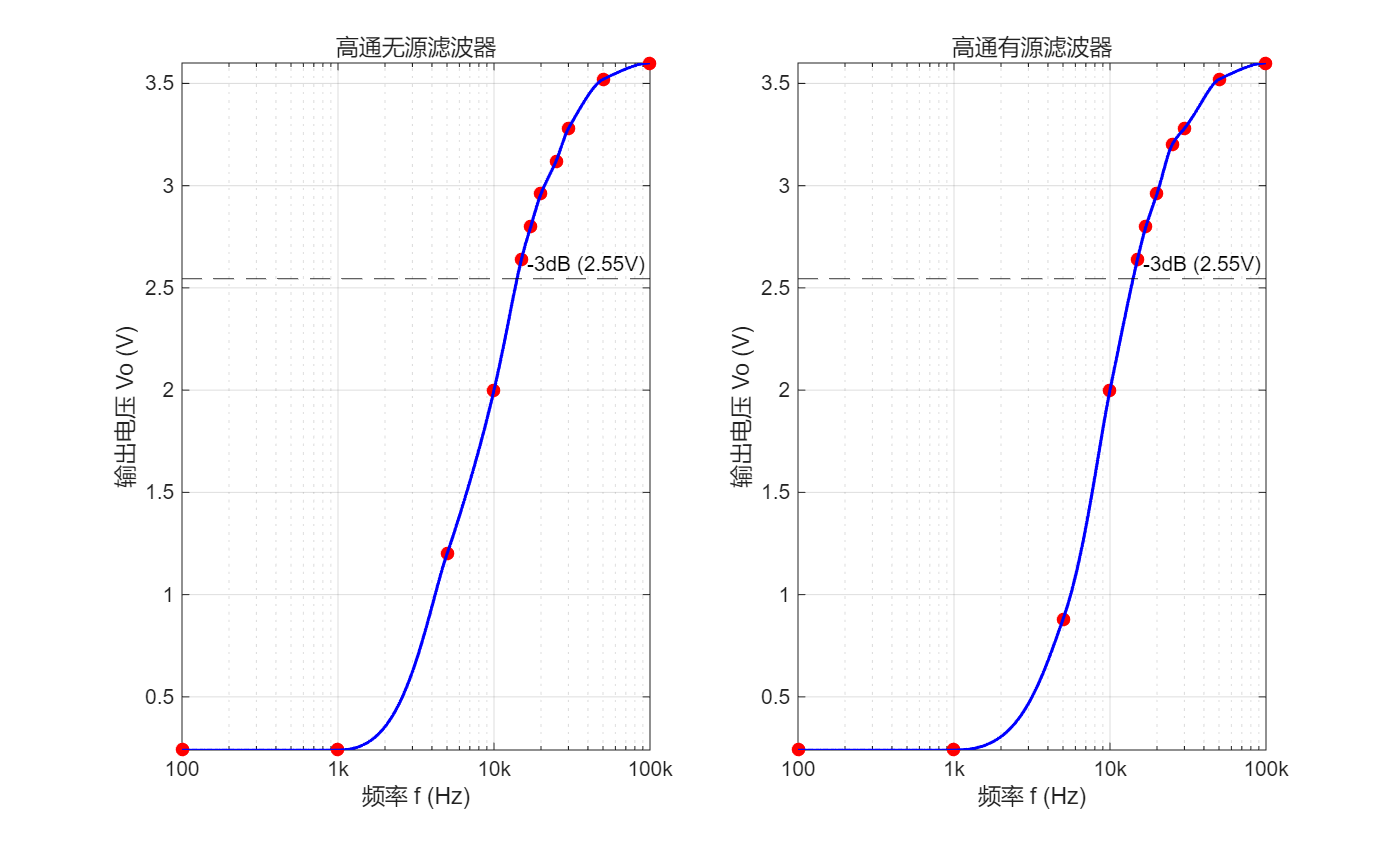
\includegraphics[width=\textwidth]{figures/高通.png}
        \caption{高通滤波器幅频特性曲线 (MATLAB)}
    \end{subfigure}
    
    \vspace{1em}
    
    \begin{subfigure}[b]{0.45\textwidth}
        \centering
        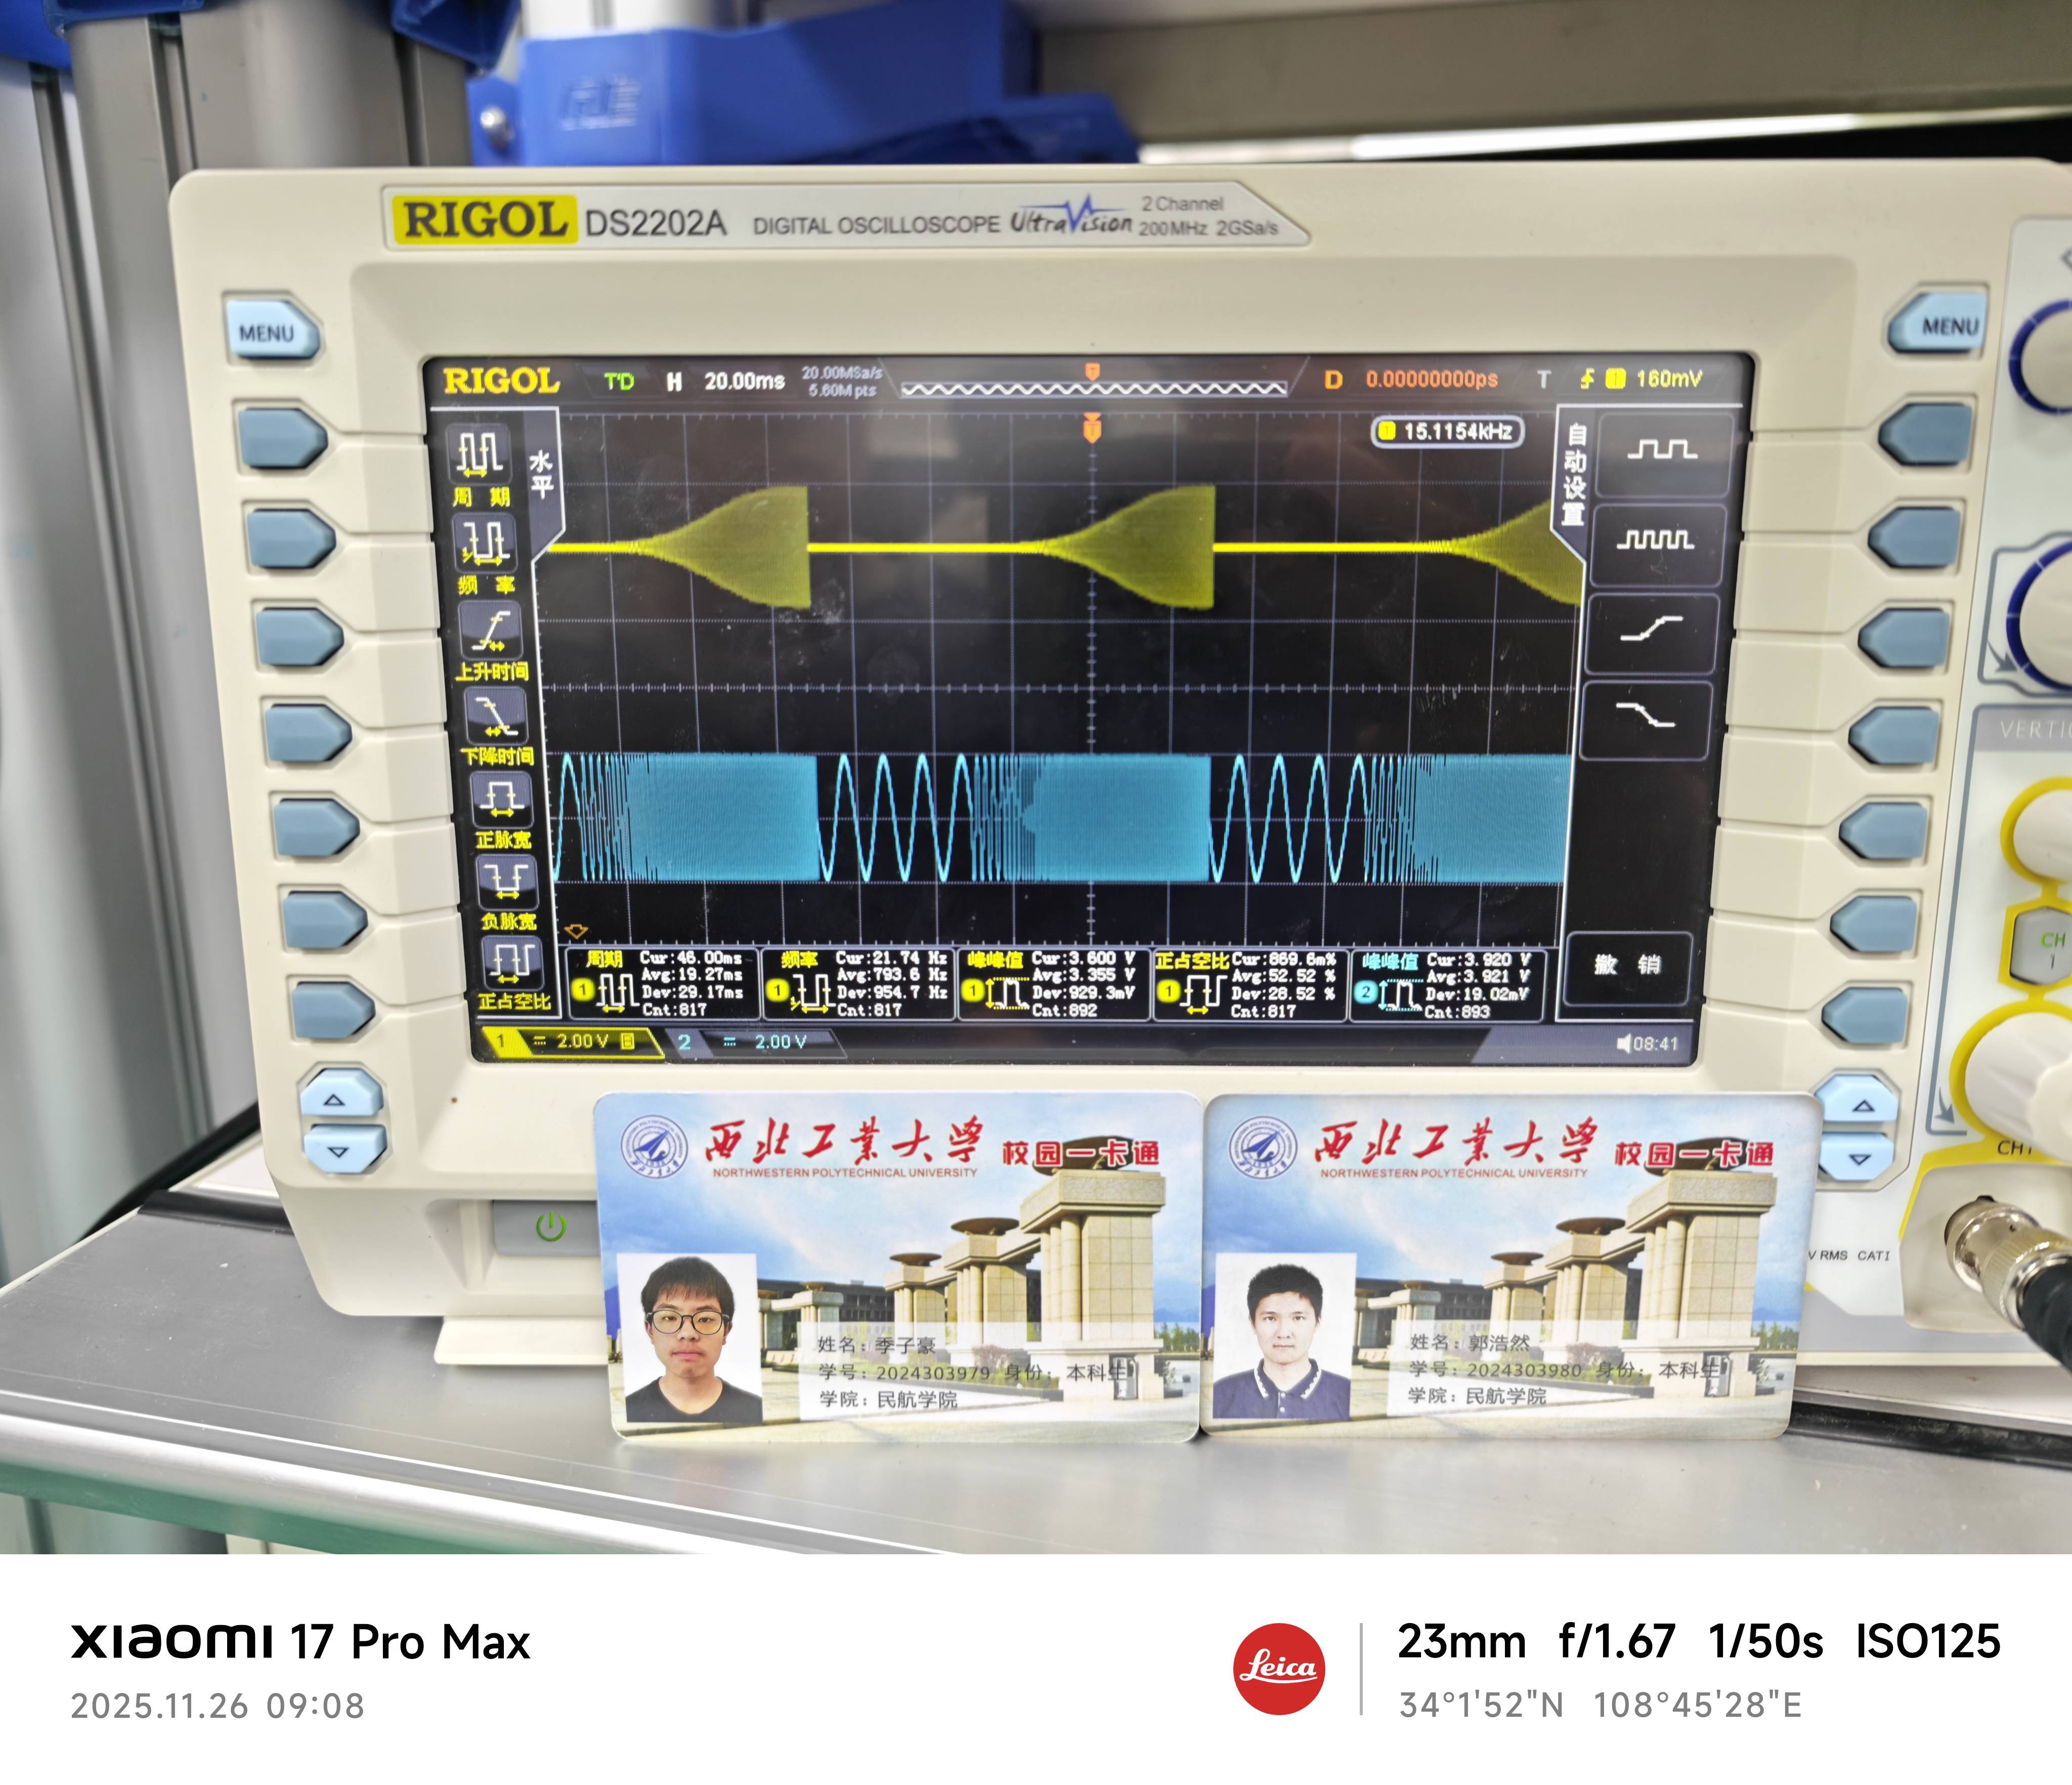
\includegraphics[width=\textwidth]{figures/无源高通.jpg}
        \caption{无源高通扫频波形}
    \end{subfigure}
    \hfill
    \begin{subfigure}[b]{0.45\textwidth}
        \centering
        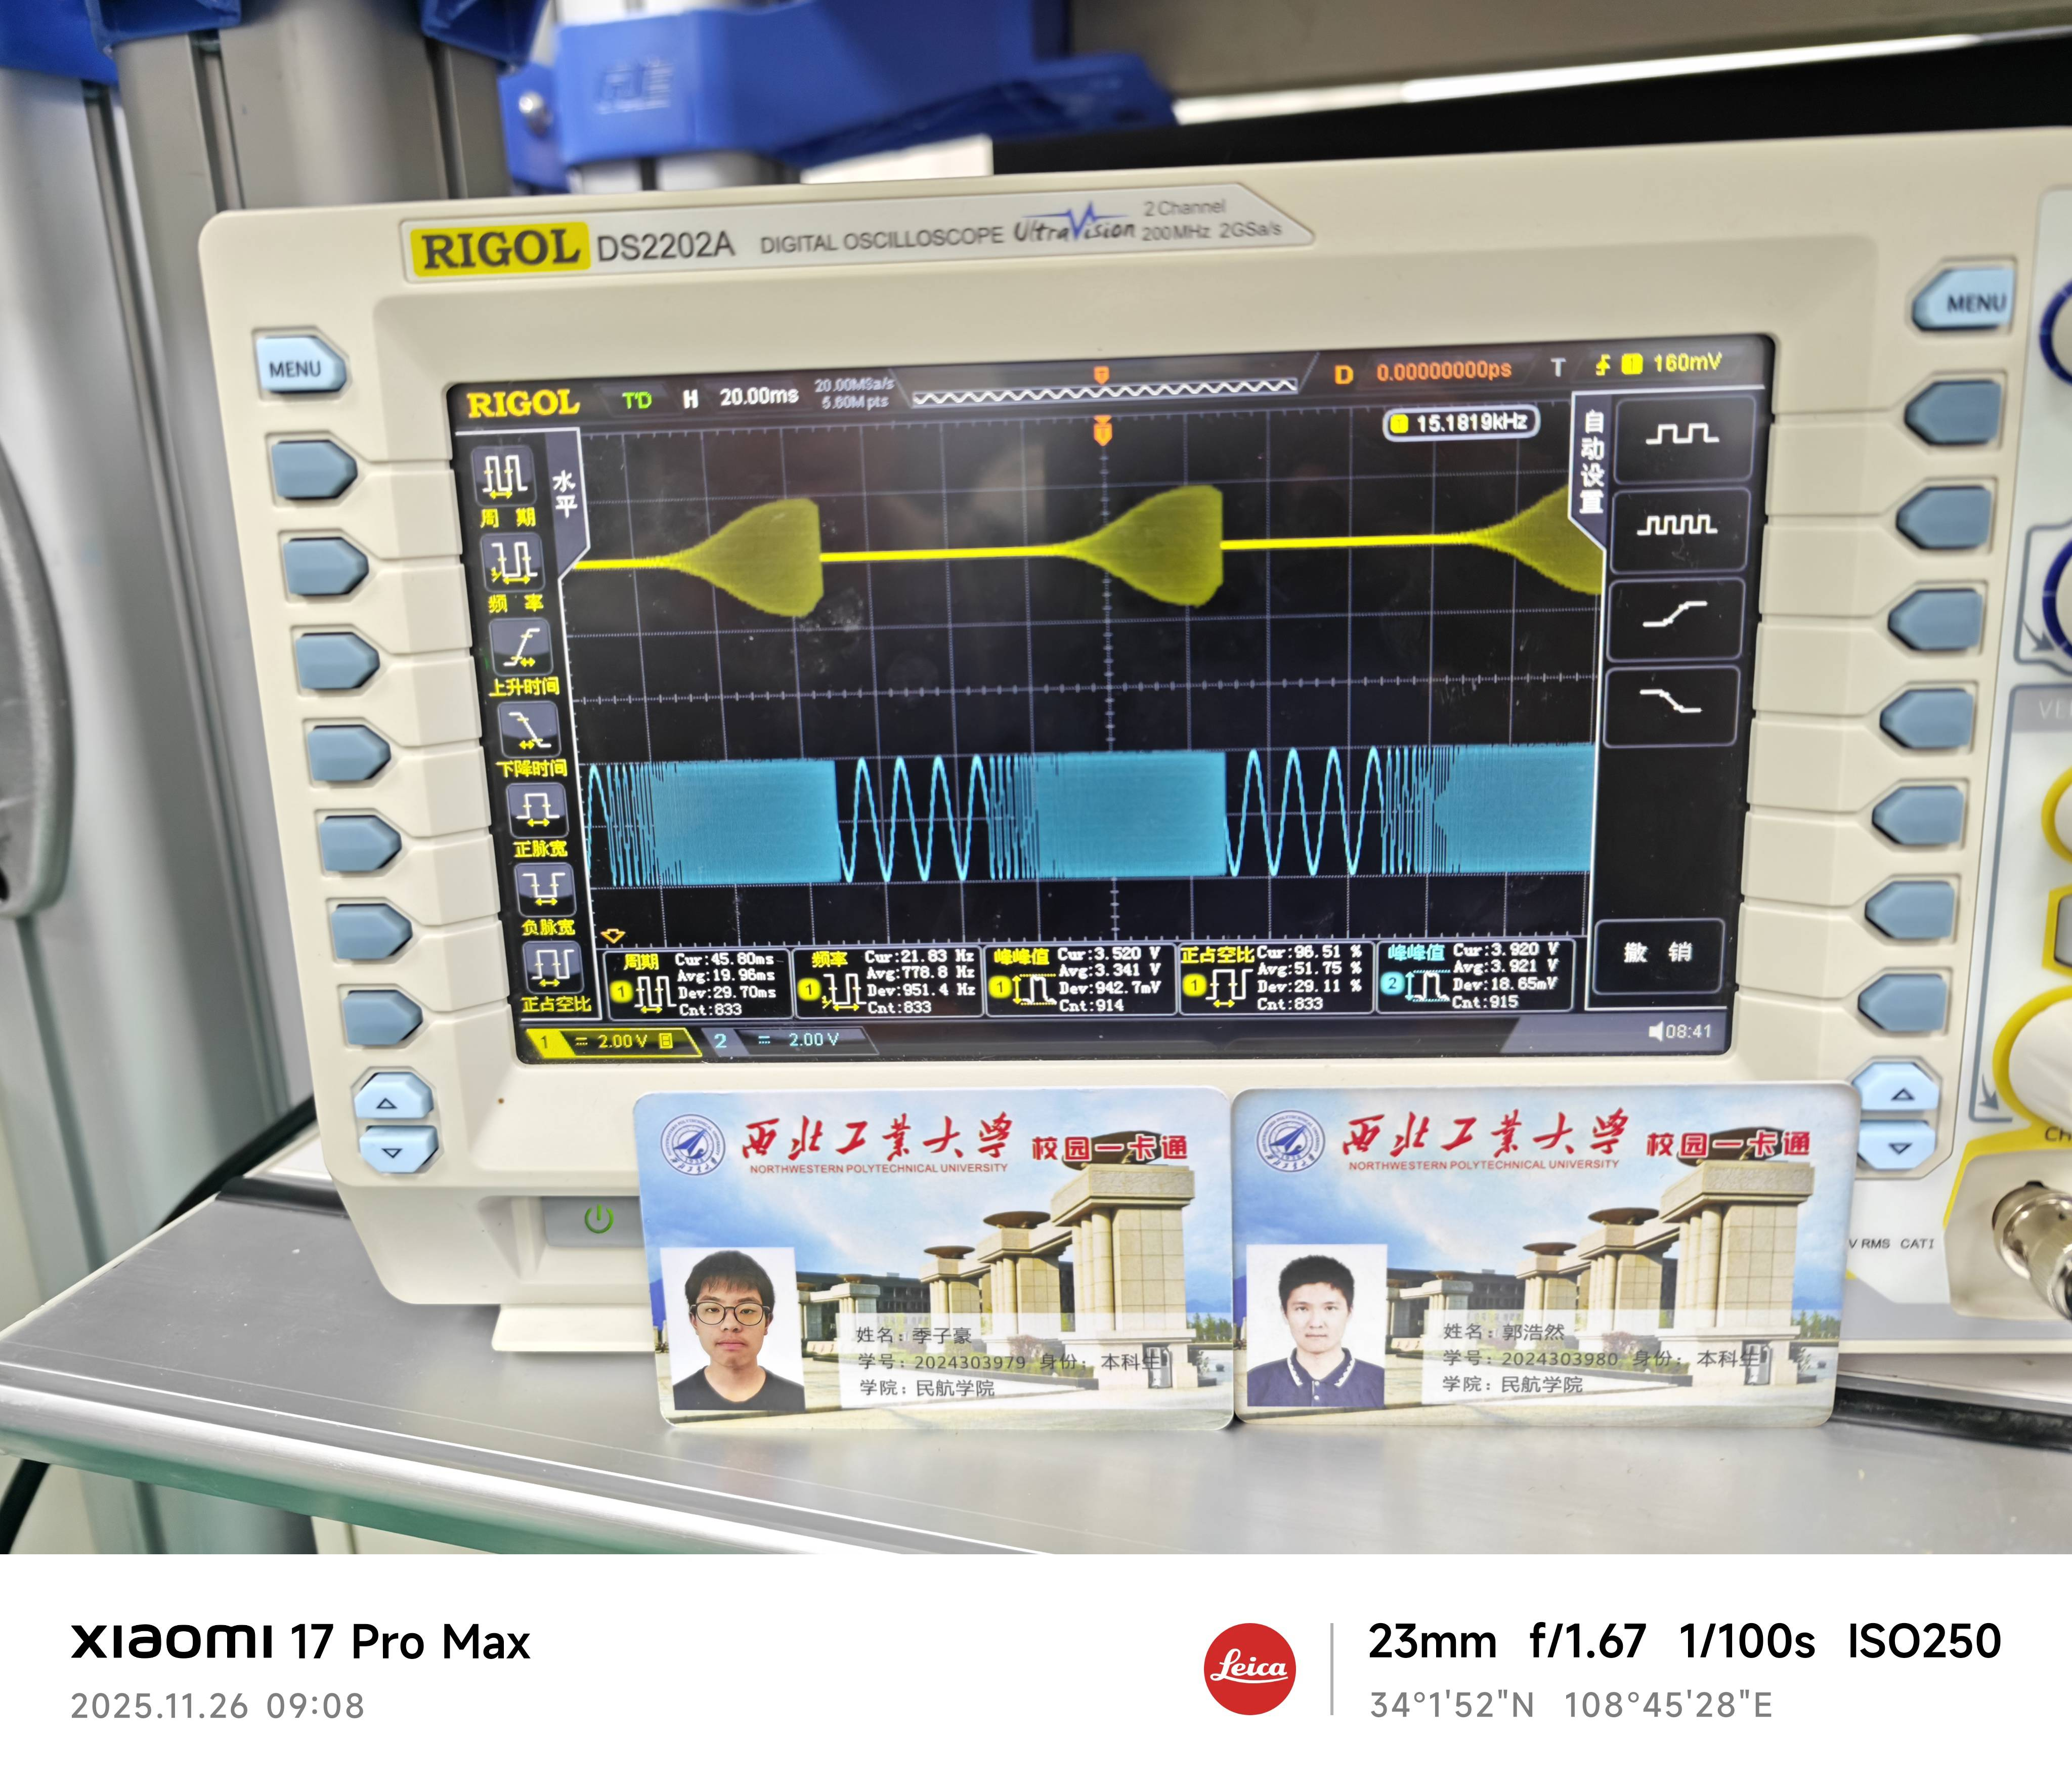
\includegraphics[width=\textwidth]{figures/有源高通.jpg}
        \caption{有源高通扫频波形}
    \end{subfigure}
    \caption{高通滤波器实验结果综合展示}
\end{figure}

\newpage

% ---------------------------------------------------------
% 任务三：带通滤波器
% ---------------------------------------------------------
\subsection{任务三：测量带通滤波器的频响特性}

\subsubsection{逐点测量法数据}

\textbf{1. 无源带通滤波器}

\mygridtable{
    \begin{tabular}{|c|c|c|c|c|c|c|c|c|c|c|c|c|}
        \hline
        $V_i$ (V) & 4 & 4 & 4 & 4 & 4 & 4 & 4 & 4 & 4 & 4 & 4 & 4 \\
        \hline
        $f$ (Hz) & 100 & 1k & \textbf{2.1k} & 5k & 10k & \textbf{13k} & 15k & 20k & 25k & 30k & 50k & 100k \\
        \hline
        $V_o$ (V) & 0.40 & 2.00 & \textbf{2.80} & 3.20 & 3.04 & \textbf{2.80} & 2.72 & 2.40 & 2.16 & 1.84 & 1.36 & 0.72 \\
        \hline
        \multicolumn{13}{|l|}{\textbf{测量结论：}  $f_L = 2.1\,\mathrm{kHz}$， $f_H = 13.0\,\mathrm{kHz}$} \\
        \hline
    \end{tabular}
}{带通无源滤波器逐点测量数据}

\textbf{2. 有源带通滤波器}

\mygridtable{
    \begin{tabular}{|c|c|c|c|c|c|c|c|c|c|c|c|}
        \hline
        $V_i$ (V) & 4 & 4 & 4 & 4 & 4 & 4 & 4 & 4 & 4 & 4 & 4 \\
        \hline
        $f$ (Hz) & 100 & 1k & \textbf{3.8k} & 5k & 10k & \textbf{15k} & 20k & 25k & 30k & 50k & 100k \\
        \hline
        $V_o$ (V) & 0.24 & 1.20 & \textbf{2.80} & 3.04 & 3.12 & \textbf{2.80} & 2.48 & 2.16 & 1.84 & 1.28 & 0.72 \\
        \hline
        \multicolumn{12}{|l|}{\textbf{测量结论：}  $f_L = 3.8\,\mathrm{kHz}$， $f_H = 15.0\,\mathrm{kHz}$} \\
        \hline
    \end{tabular}
}{带通有源滤波器逐点测量数据}

\subsubsection{幅频特性曲线与扫频测试}

\begin{figure}[H]
    \centering
    \begin{subfigure}[b]{0.8\textwidth}
        \centering
        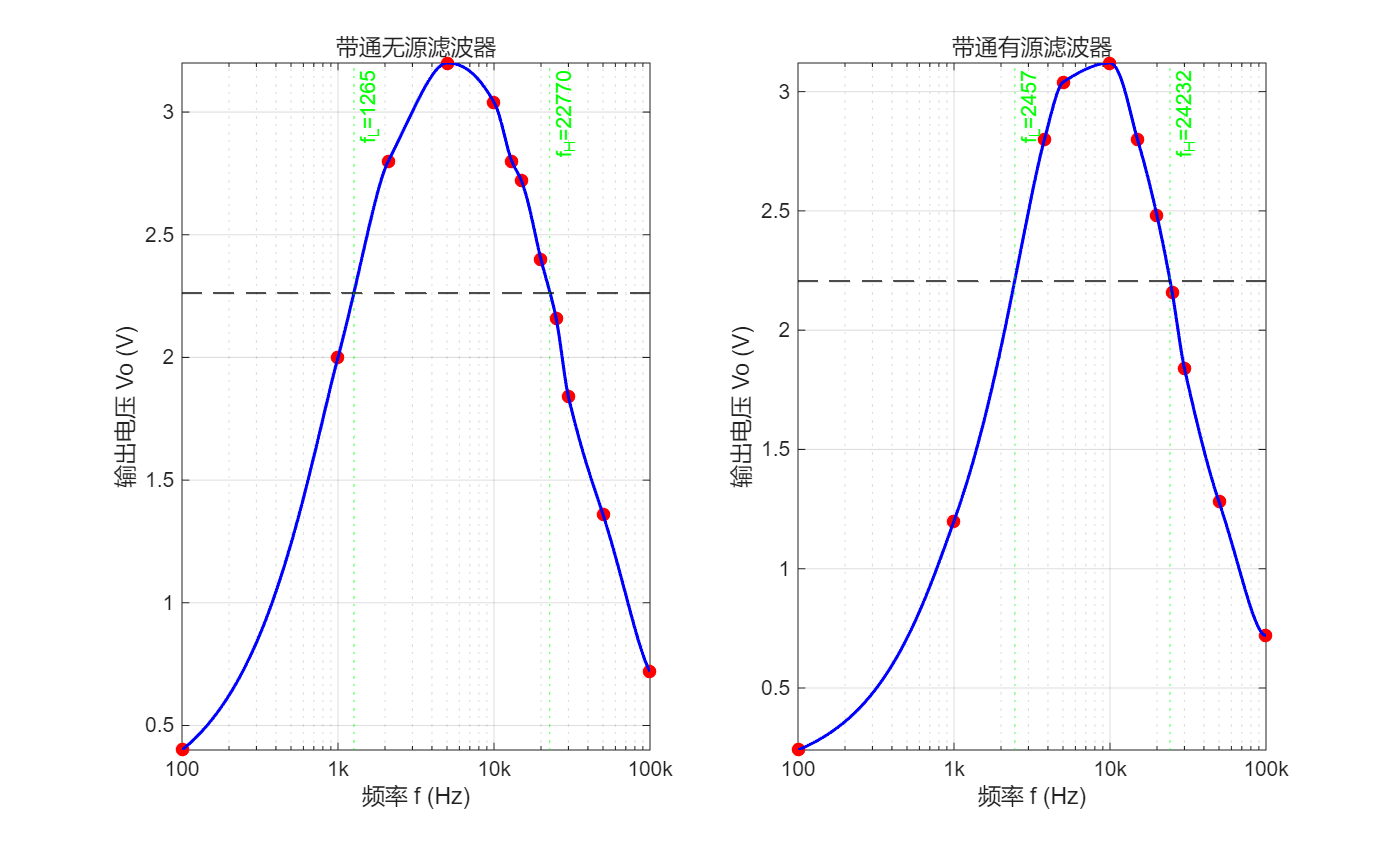
\includegraphics[width=\textwidth]{figures/带通.png}
        \caption{带通滤波器幅频特性曲线 (MATLAB)}
    \end{subfigure}
    
    \vspace{1em}
    
    \begin{subfigure}[b]{0.45\textwidth}
        \centering
        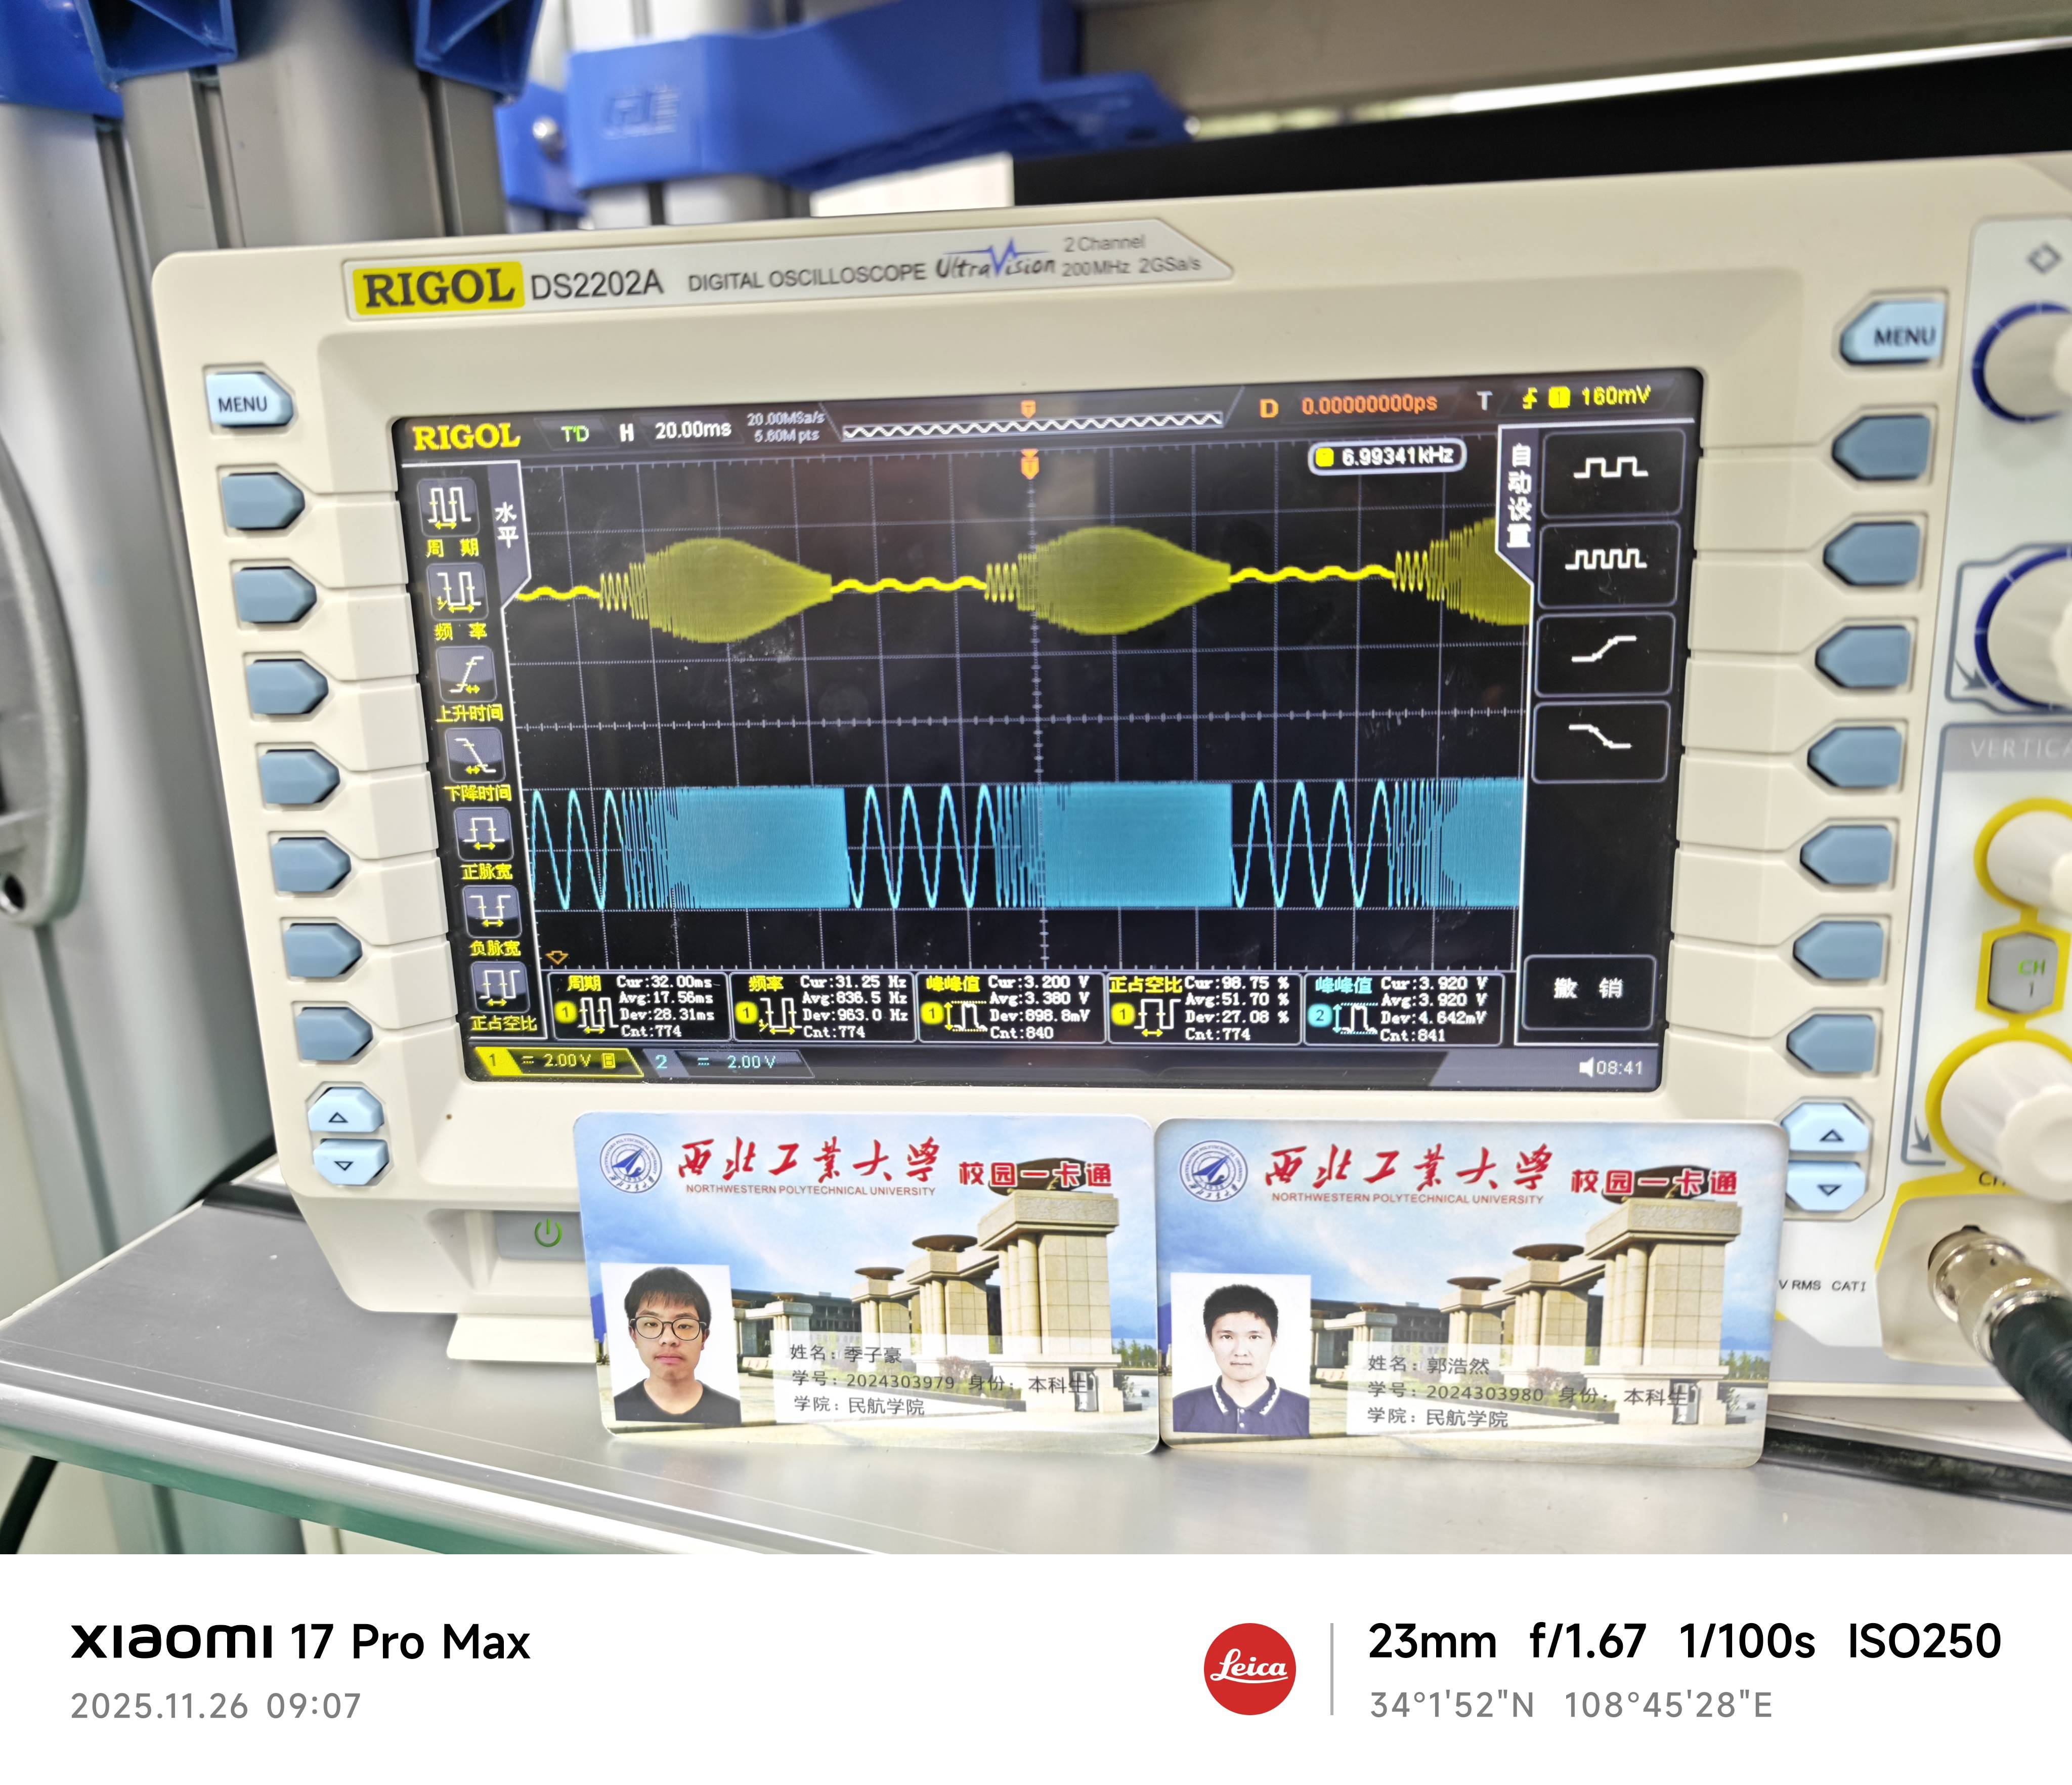
\includegraphics[width=\textwidth]{figures/无源带通.jpg}
        \caption{无源带通扫频波形}
    \end{subfigure}
    \hfill
    \begin{subfigure}[b]{0.45\textwidth}
        \centering
        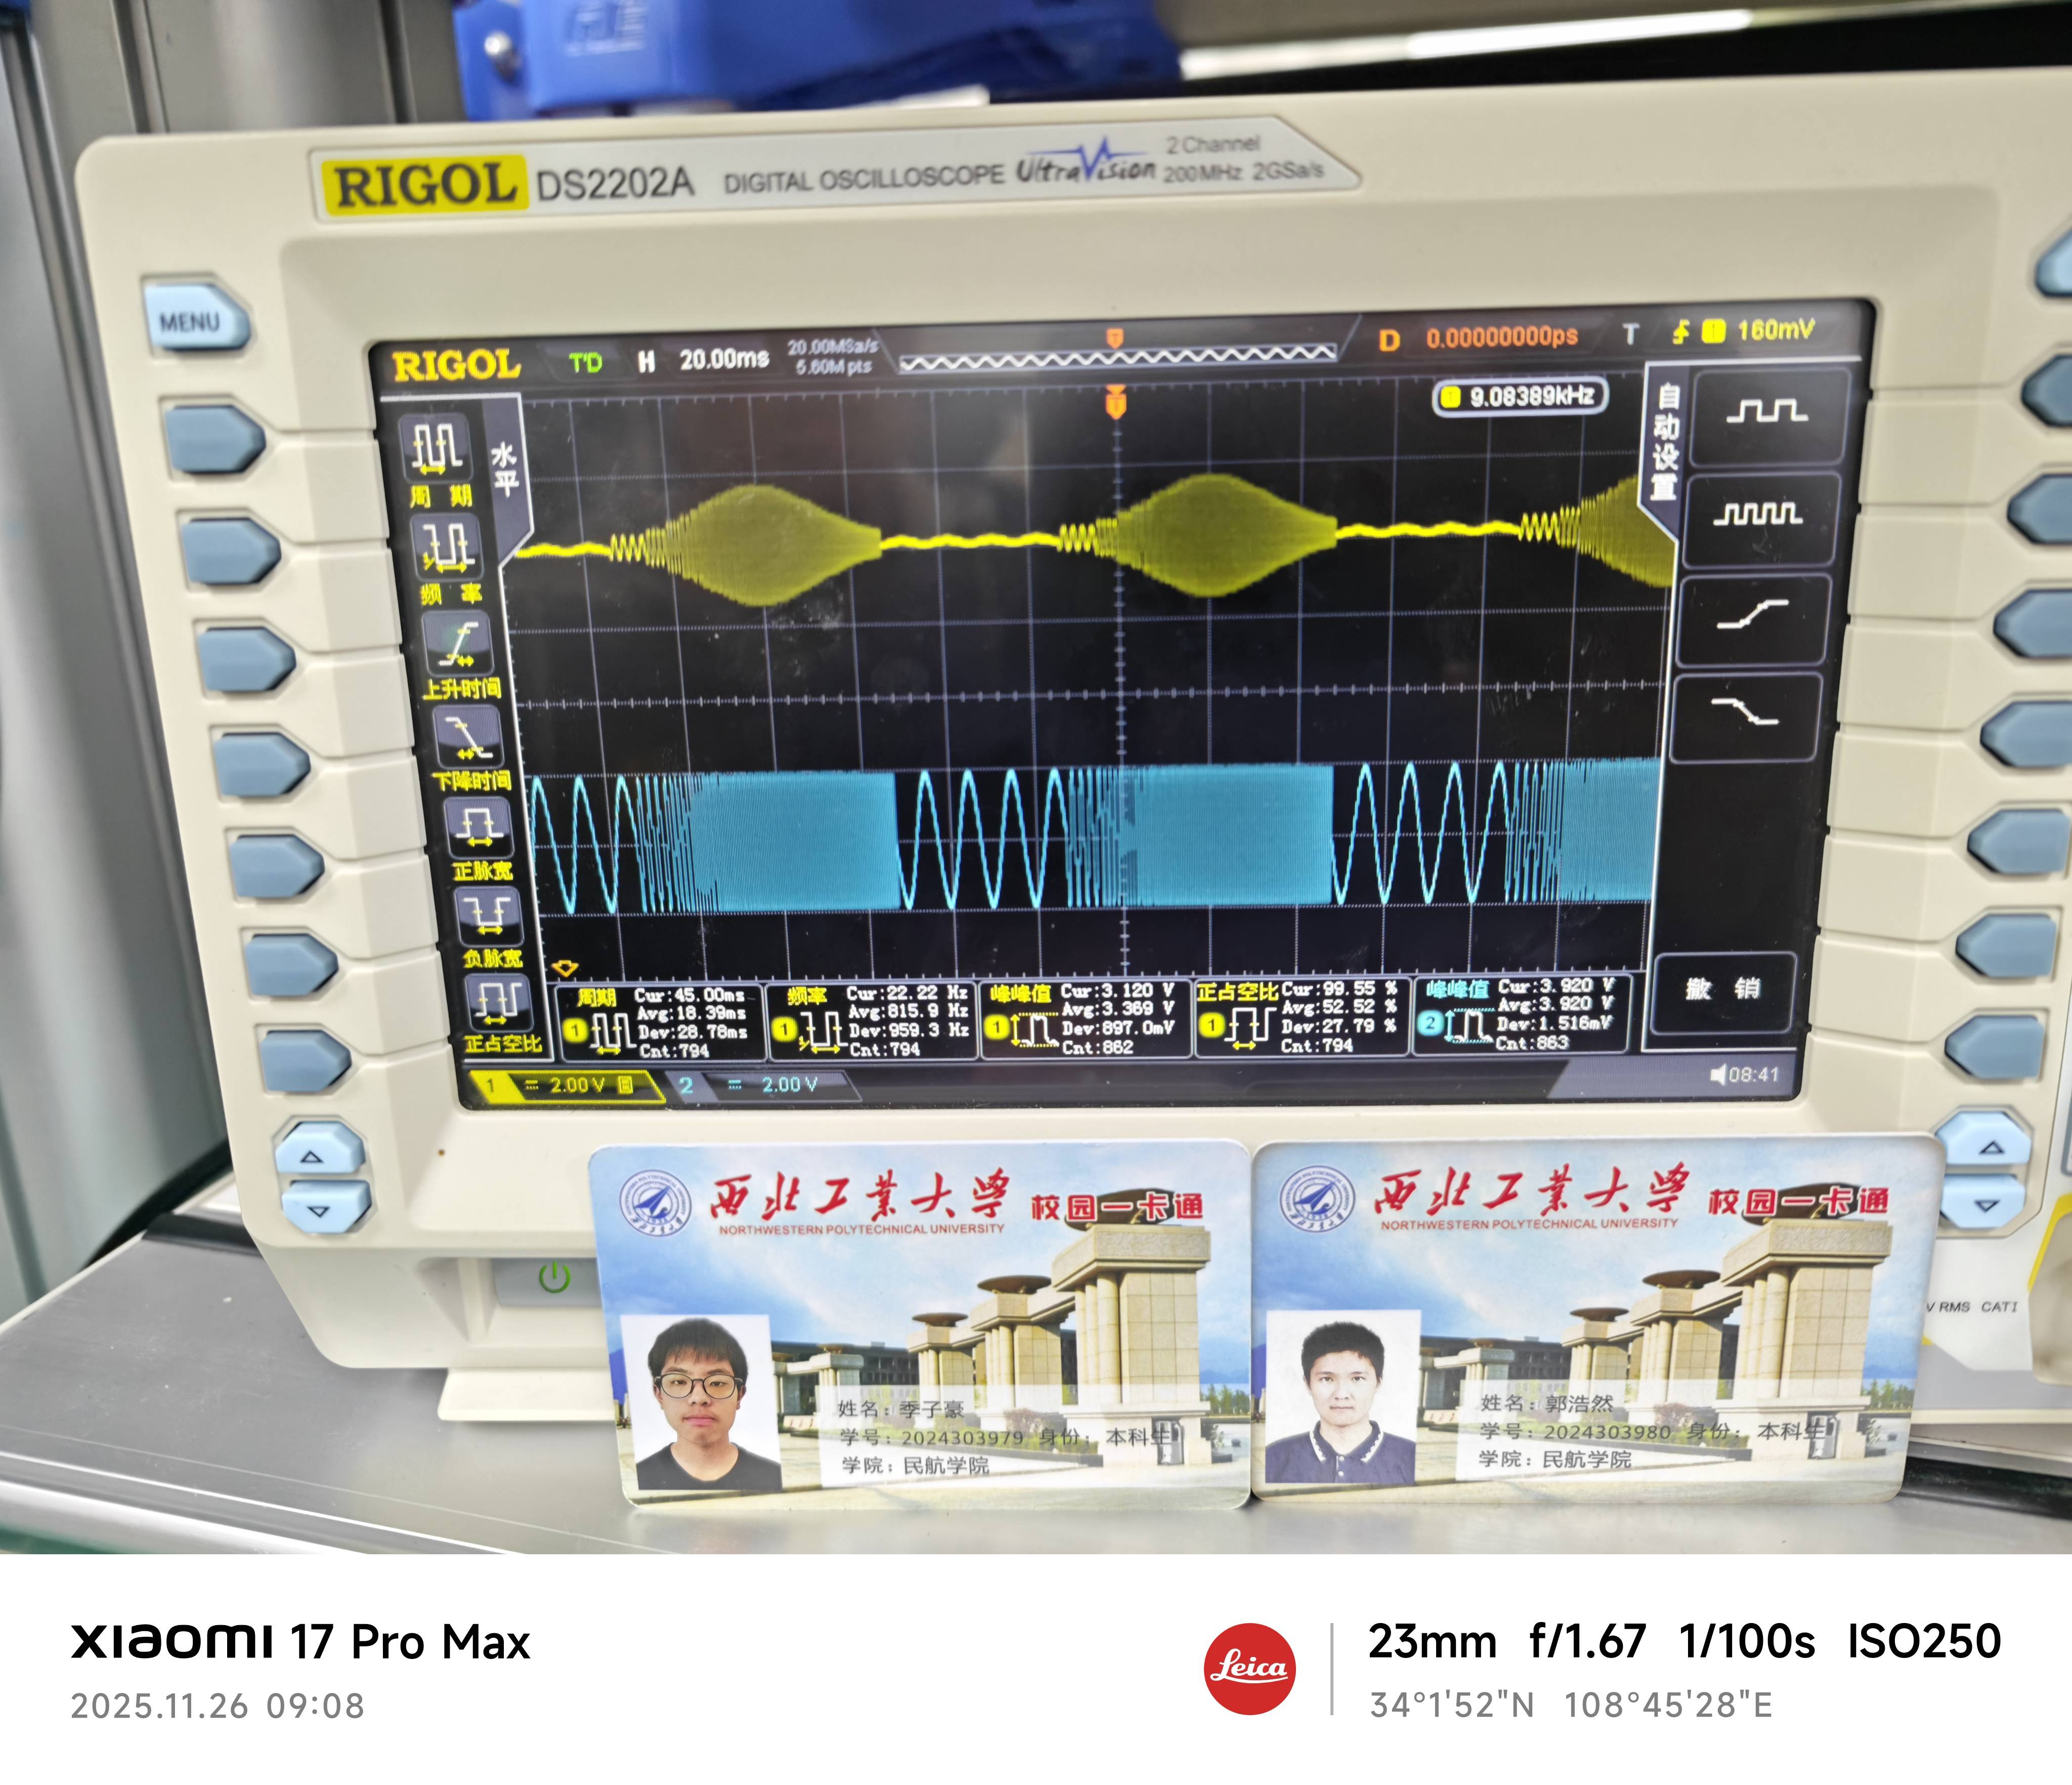
\includegraphics[width=\textwidth]{figures/有源带通.jpg}
        \caption{有源带通扫频波形}
    \end{subfigure}
    \caption{带通滤波器实验结果综合展示}
\end{figure}

\newpage

% ---------------------------------------------------------
% 任务四：带阻滤波器
% ---------------------------------------------------------
\subsection{任务四：测量带阻滤波器的频响特性}

\subsubsection{逐点测量法数据}

\textbf{1. 无源带阻滤波器}

\mygridtable{
    \begin{tabular}{|c|c|c|c|c|c|c|c|c|c|c|c|c|c|c|c|c|c|}
        \hline
        $V_i$ (V) & 4 & 4 & 4 & 4 & 4 & 4 & 4 & 4 & 4 & 4 & 4 & 4 & 4 & 4 & 4 & 4 & 4 \\
        \hline
        $f$ (Hz) & 100 & 500 & 1k & 3k & \textbf{3.6k} & 5k & 10k & 15k & 20k & 25k & 30k & 40k & 50k & 60k & 80k & \textbf{85k} & 100k \\
        \hline
        $V_o$ (V) & 3.84 & 3.84 & 3.68 & 3.04 & \textbf{2.80} & 2.32 & 1.04 & 0.32 & 0.48 & 0.88 & 1.28 & 1.76 & 2.08 & 2.40 & 2.72 & \textbf{2.80} & 2.96 \\
        \hline
        \multicolumn{18}{|l|}{\textbf{测量结论：}  $f_L = 3.6\,\mathrm{kHz}$， $f_H = 85.0\,\mathrm{kHz}$} \\
        \hline
    \end{tabular}
}{带阻无源滤波器逐点测量数据}

\textbf{2. 有源带阻滤波器}

\mygridtable{
    \begin{tabular}{|c|c|c|c|c|c|c|c|c|c|c|c|c|c|c|}
        \hline
        $V_i$ (V) & 4 & 4 & 4 & 4 & 4 & 4 & 4 & 4 & 4 & 4 & 4 & 4 & 4 & 4 \\
        \hline
        $f$ (Hz) & 100 & 500 & 1k & 3k & 5k & \textbf{6.5k} & 10k & 15k & 20k & 25k & 30k & \textbf{45.8k} & 50k & 80k \\
        \hline
        $V_o$ (V) & 3.92 & 3.84 & 3.84 & 3.52 & 3.12 & \textbf{2.80} & 1.76 & 0.48 & 0.88 & 1.60 & 2.08 & \textbf{2.80} & 2.88 & 2.96 \\
        \hline
        \multicolumn{15}{|l|}{\textbf{测量结论：}  $f_L = 6.5\,\mathrm{kHz}$， $f_H = 45.8\,\mathrm{kHz}$} \\
        \hline
    \end{tabular}
}{带阻有源滤波器逐点测量数据}

\subsubsection{幅频特性曲线与扫频测试}

\begin{figure}[H]
    \centering
    \begin{subfigure}[b]{0.8\textwidth}
        \centering
        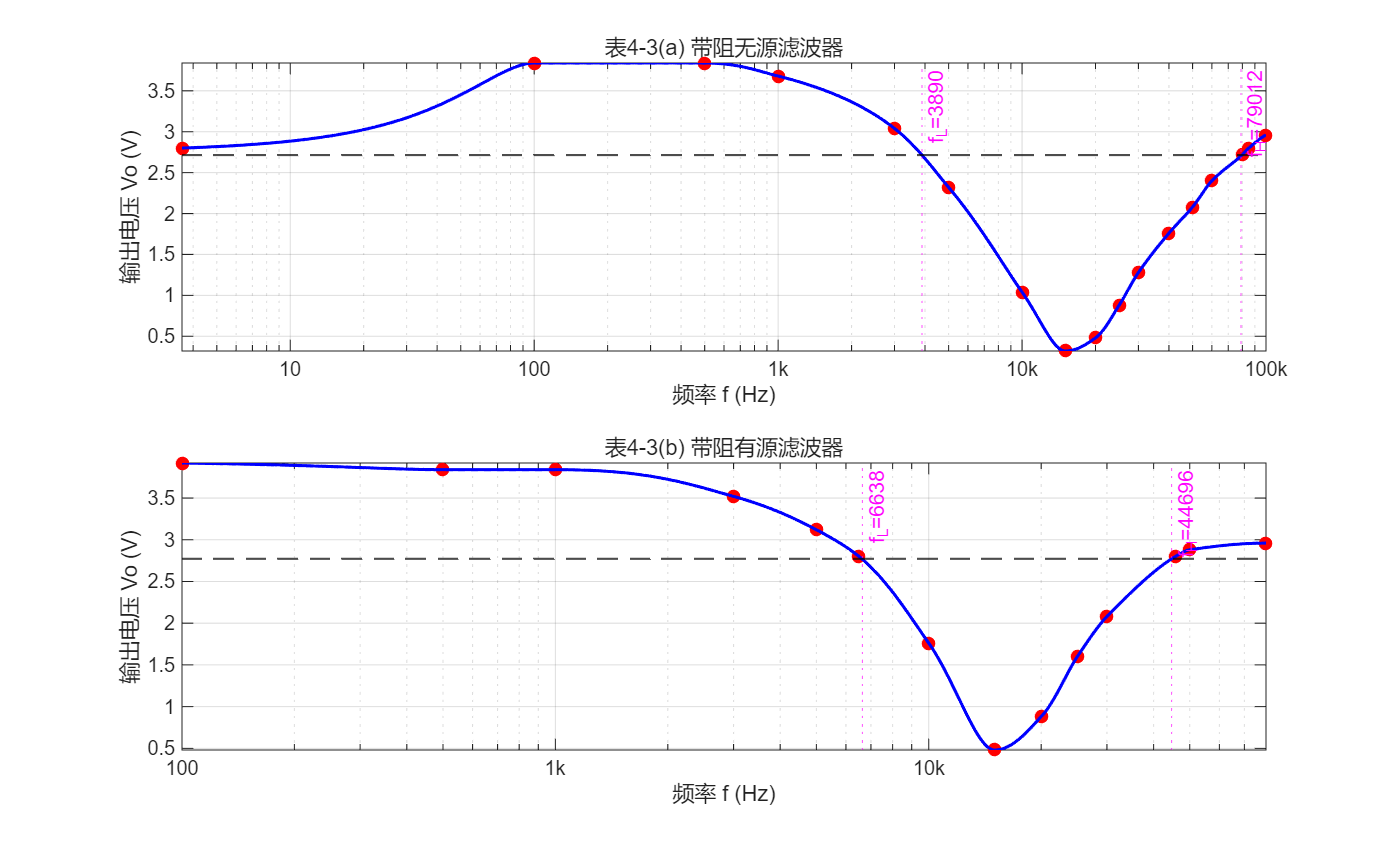
\includegraphics[width=\textwidth]{figures/带阻.png}
        \caption{带阻滤波器幅频特性曲线 (MATLAB)}
    \end{subfigure}
    
    \vspace{1em}
    
    \begin{subfigure}[b]{0.45\textwidth}
        \centering
        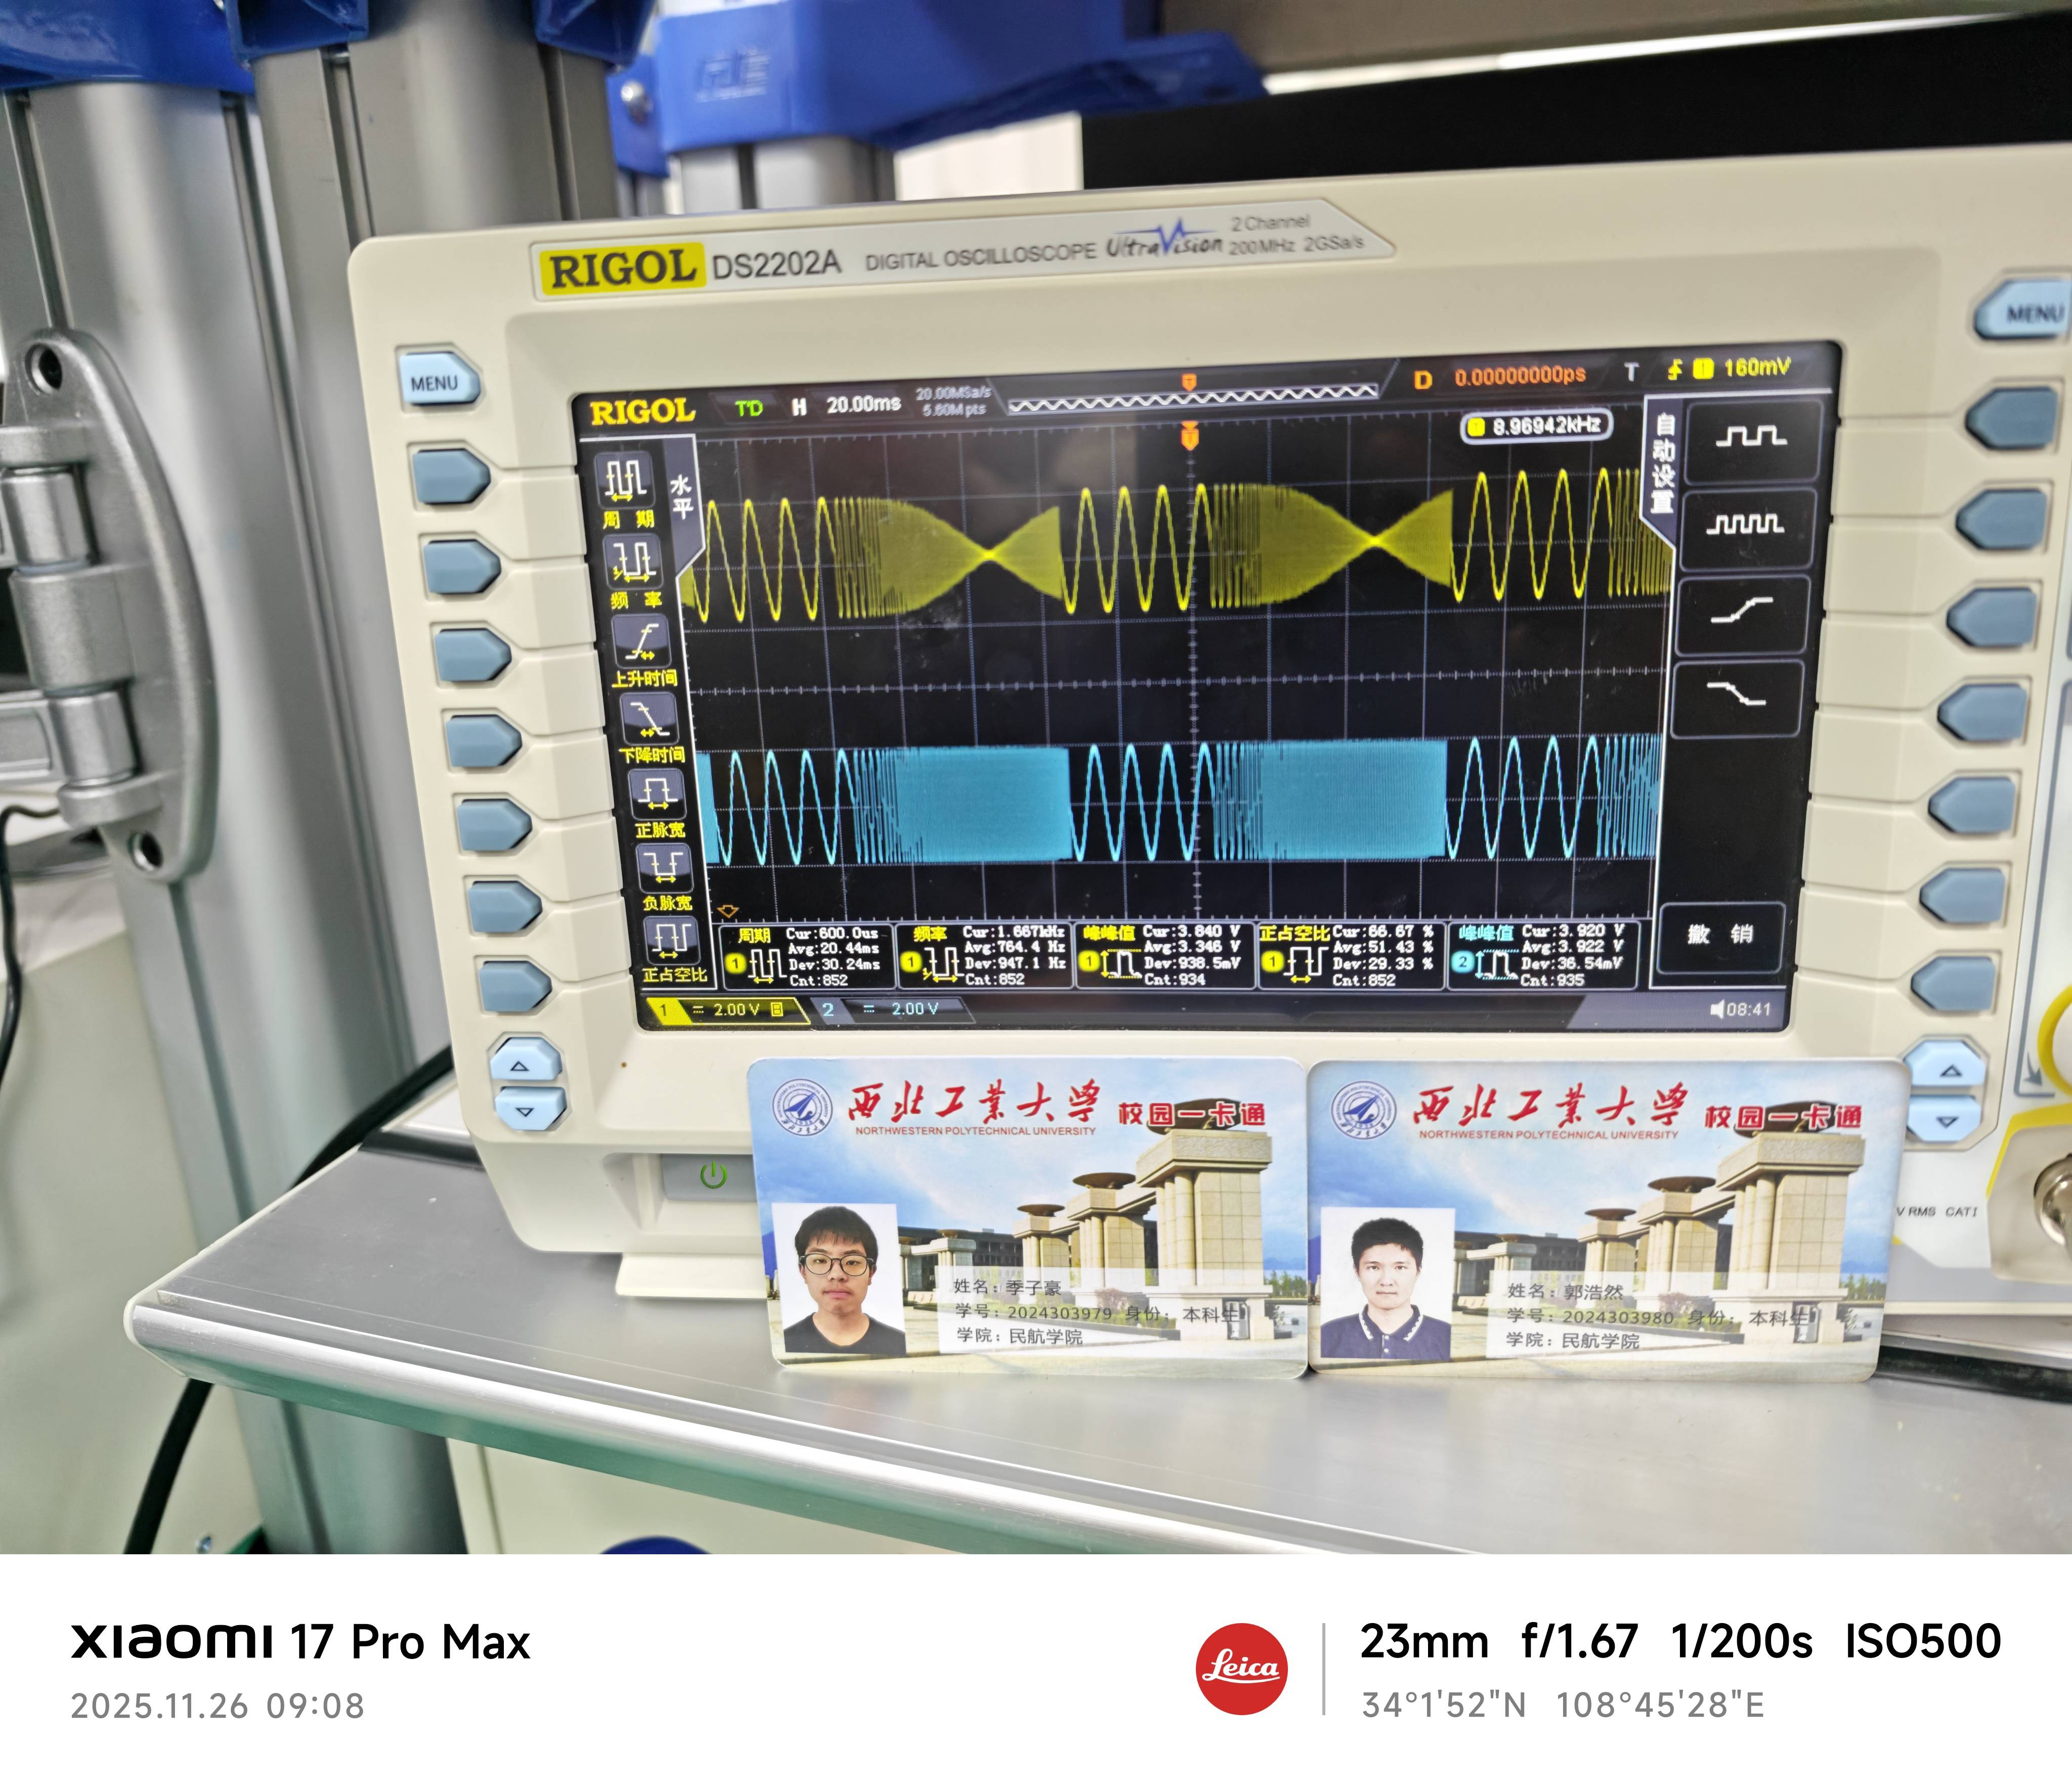
\includegraphics[width=\textwidth]{figures/无源带阻.jpg}
        \caption{无源带阻扫频波形}
    \end{subfigure}
    \hfill
    \begin{subfigure}[b]{0.45\textwidth}
        \centering
        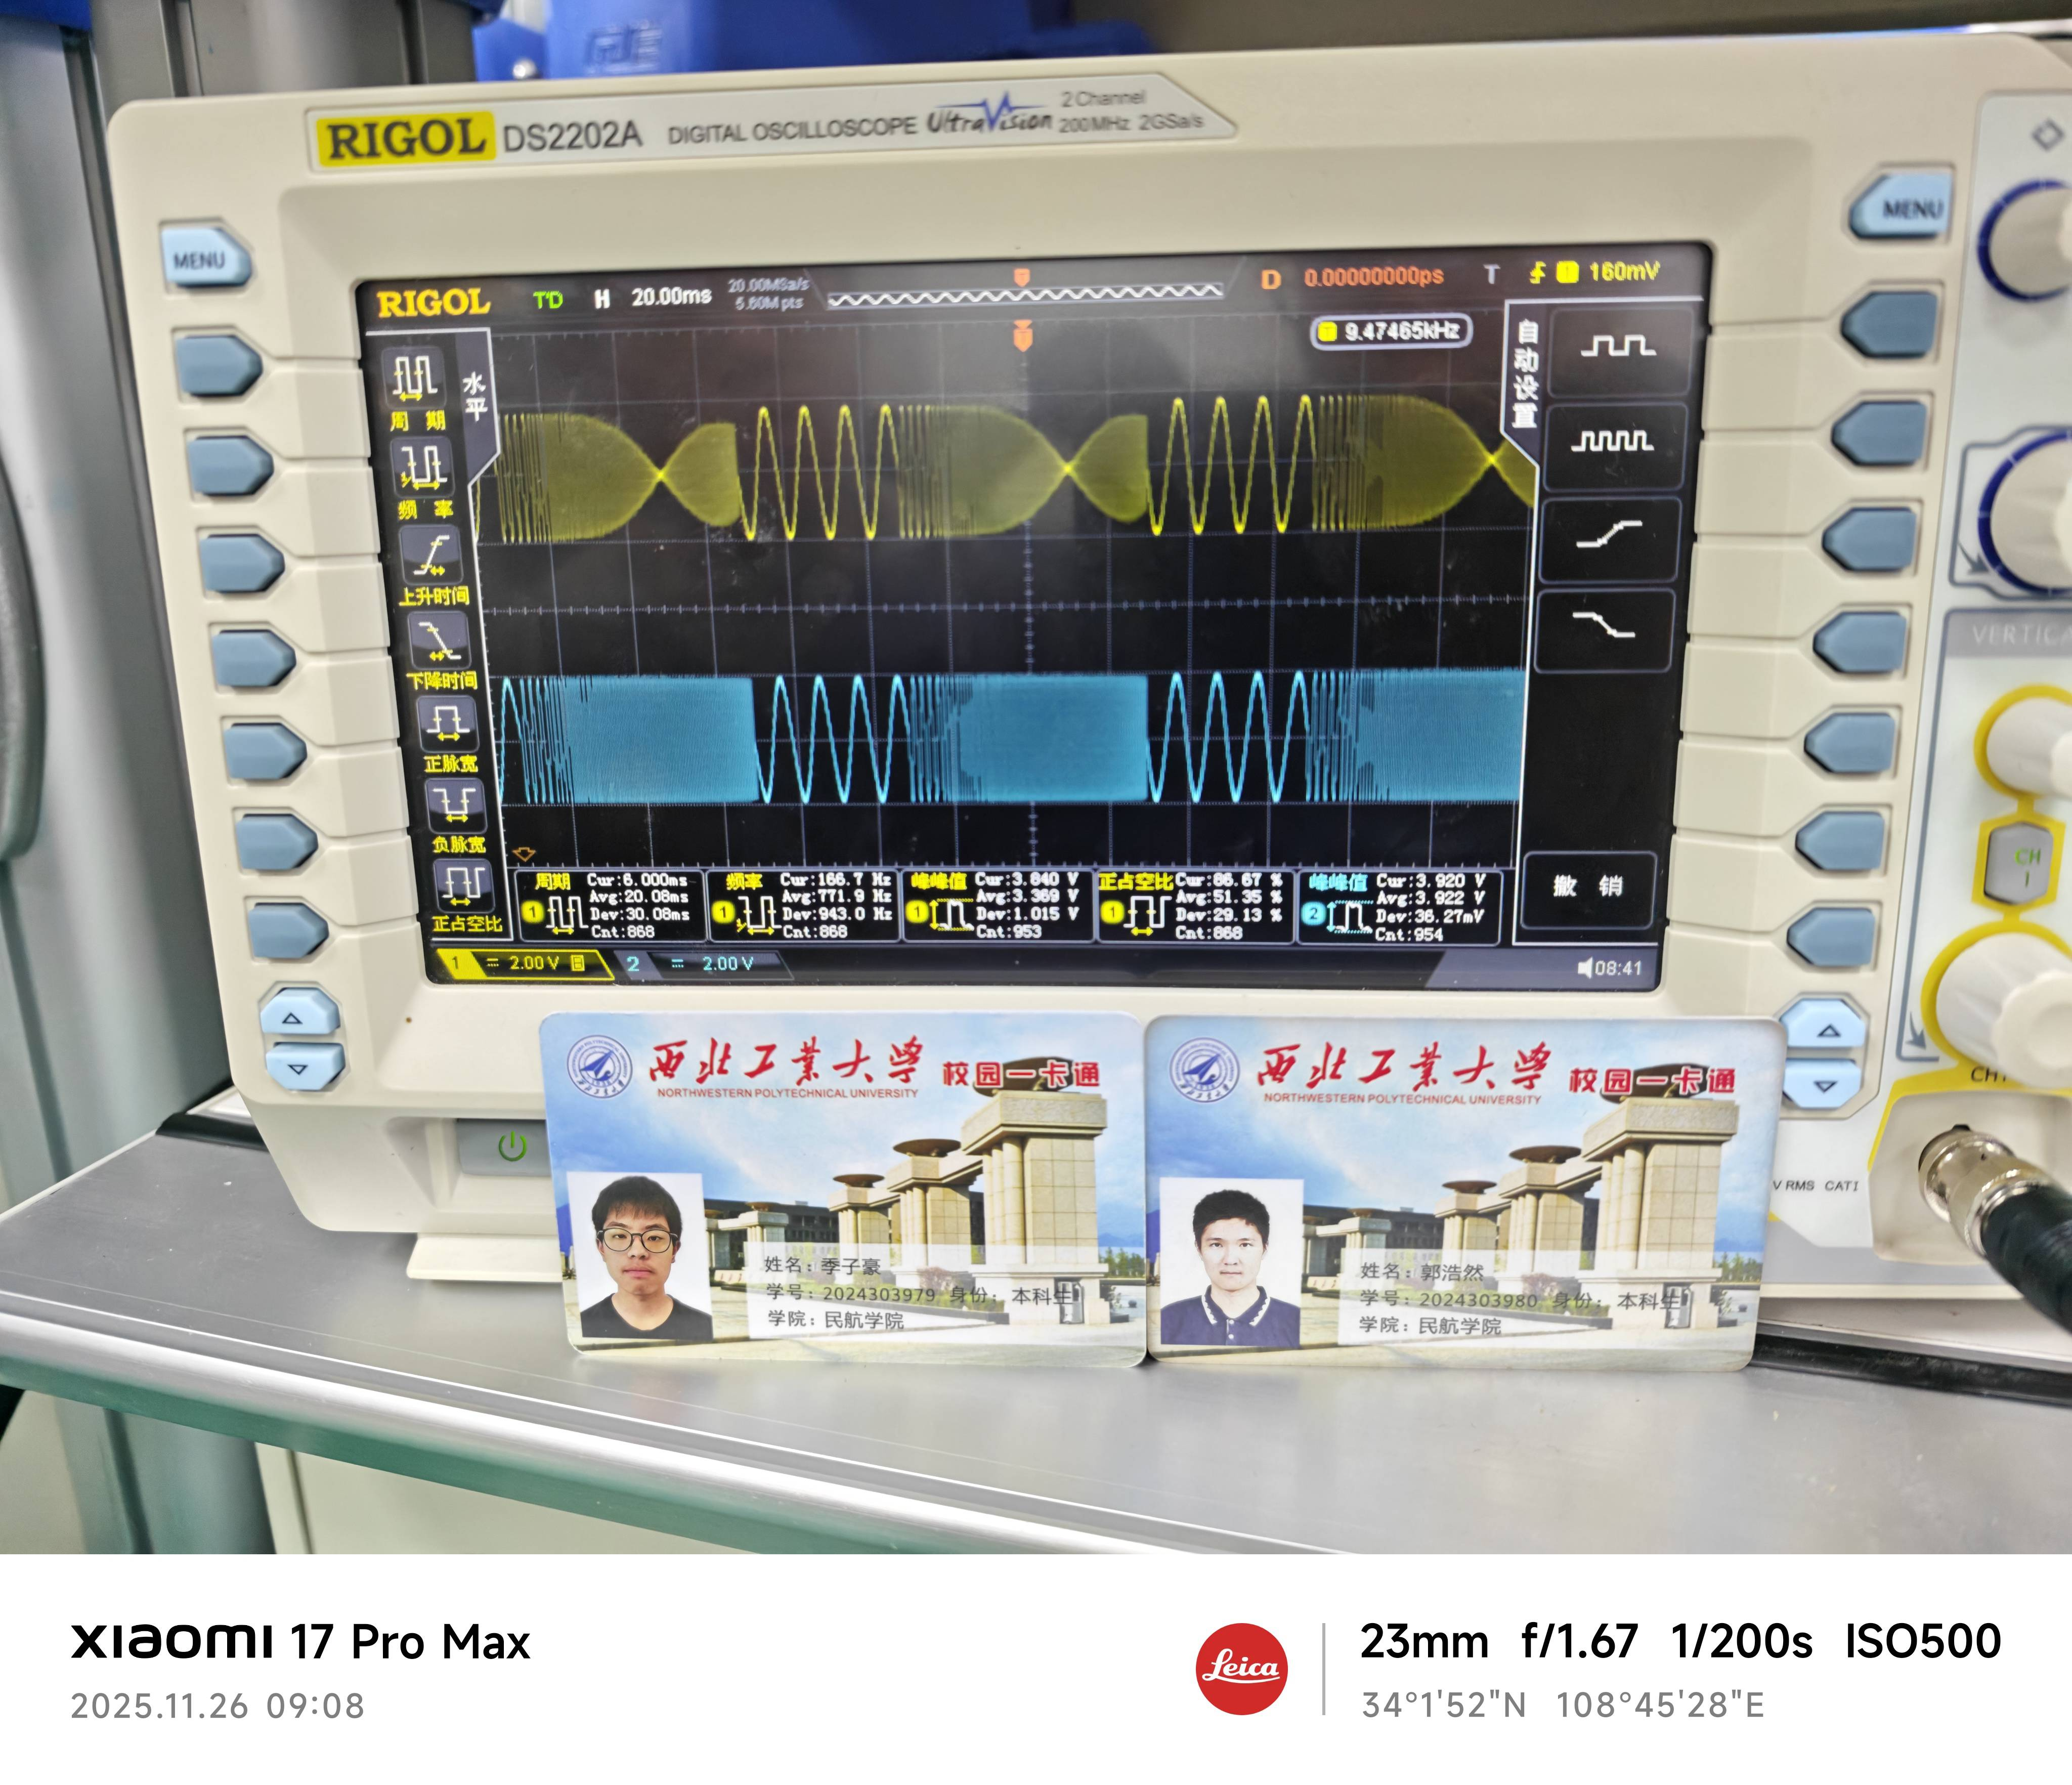
\includegraphics[width=\textwidth]{figures/有源带阻.jpg}
        \caption{有源带阻扫频波形}
    \end{subfigure}
    \caption{带阻滤波器实验结果综合展示}
\end{figure}

\newpage

% ==========================================
% 第三部分：实验总结与心得
% ==========================================

\section{实验总结与心得}

\subsection{实验数据汇总}

经过对有源、无源滤波器（低通、高通、带通、带阻）的逐点测量与扫频测试，最终测得的截止频率参数汇总如表 \ref{tab:final_result} 所示。

\begin{table}[H]
    \centering
    \renewcommand{\arraystretch}{1.5}
    \setlength{\tabcolsep}{8pt}
    \begin{tabular}{|l|l|l|}
        \hline
        \textbf{类型} & \textbf{无源参数} & \textbf{有源参数} \\
        \hline
        低通 & $f_H = 18.5\,\mathrm{kHz}$ & $f_H = 16.7\,\mathrm{kHz}$ \\
        高通 & $f_L = 17.2\,\mathrm{kHz}$ & $f_L = 17.0\,\mathrm{kHz}$ \\
        \hline
        带通 & \makecell[l]{$f_L = 2.1\,\mathrm{kHz}$ \\ $f_H = 13.0\,\mathrm{kHz}$} &
               \makecell[l]{$f_L = 3.8\,\mathrm{kHz}$ \\ $f_H = 15.0\,\mathrm{kHz}$} \\
        \hline
        带阻 & \makecell[l]{$f_L = 3.6\,\mathrm{kHz}$ \\ $f_H = 85.0\,\mathrm{kHz}$} &
               \makecell[l]{$f_L = 6.5\,\mathrm{kHz}$ \\ $f_H = 45.8\,\mathrm{kHz}$} \\
        \hline
    \end{tabular}
    \caption{滤波器截止频率测量结果汇总}
    \label{tab:final_result}
\end{table}


\subsection{实验心得}

通过本次实验，我深入理解了有源与无源滤波器的基本构成及其频率响应特性。
\begin{enumerate}
    \item \textbf{测量方法的掌握}：熟练掌握了“逐点测量法”和“扫频法”两种测量幅频特性的手段。逐点法虽然繁琐，但能提供精确的量化数据，便于计算截止频率；扫频法则能直观、快速地在示波器上显示出滤波器的整体频响曲线，便于定性分析。
    \item \textbf{理论与实践的结合}：实验中观察到的幅频特性曲线与理论分析基本一致。例如，低通滤波器在高频段的衰减、带通滤波器的选频特性等都在实验中得到了验证。同时，也观察到了实际元器件参数误差对截止频率的影响，这提示我们在工程实践中需要考虑元器件的容差。
    \item \textbf{有源与无源的对比}：通过对比发现，有源滤波器由于引入了运放，具有一定的信号放大能力（通带增益可能大于1），且负载效应较小；而无源滤波器结构简单，但信号经过后会有一定的衰减。
\end{enumerate}

本次实验不仅锻炼了我的动手操作能力，也加深了我对信号处理中滤波概念的理解，为后续课程的学习打下了良好的基础。

\end{document}


\end{document}